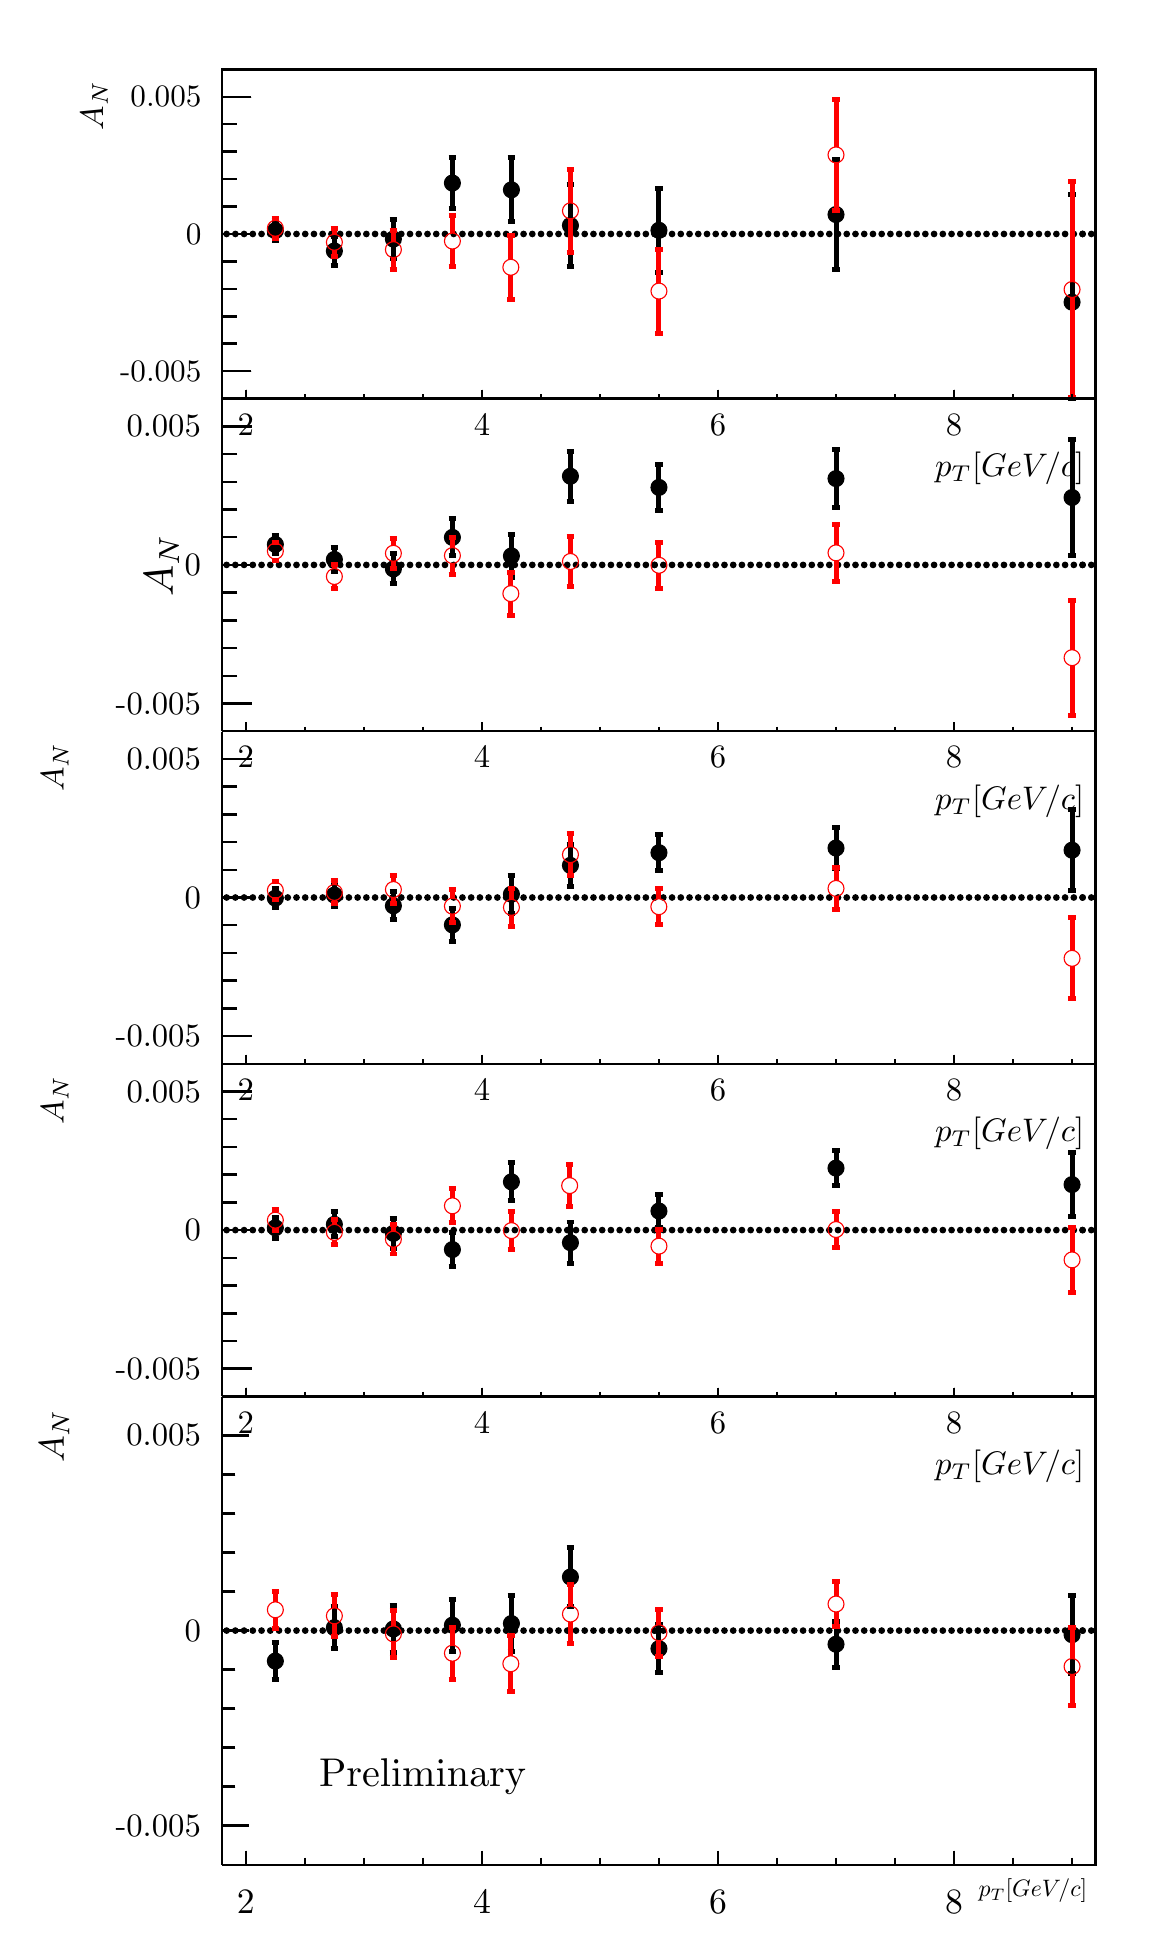
\begin{tikzpicture}
\pgfdeclareplotmark{cross} {
\pgfpathmoveto{\pgfpoint{-0.3\pgfplotmarksize}{\pgfplotmarksize}}
\pgfpathlineto{\pgfpoint{+0.3\pgfplotmarksize}{\pgfplotmarksize}}
\pgfpathlineto{\pgfpoint{+0.3\pgfplotmarksize}{0.3\pgfplotmarksize}}
\pgfpathlineto{\pgfpoint{+1\pgfplotmarksize}{0.3\pgfplotmarksize}}
\pgfpathlineto{\pgfpoint{+1\pgfplotmarksize}{-0.3\pgfplotmarksize}}
\pgfpathlineto{\pgfpoint{+0.3\pgfplotmarksize}{-0.3\pgfplotmarksize}}
\pgfpathlineto{\pgfpoint{+0.3\pgfplotmarksize}{-1.\pgfplotmarksize}}
\pgfpathlineto{\pgfpoint{-0.3\pgfplotmarksize}{-1.\pgfplotmarksize}}
\pgfpathlineto{\pgfpoint{-0.3\pgfplotmarksize}{-0.3\pgfplotmarksize}}
\pgfpathlineto{\pgfpoint{-1.\pgfplotmarksize}{-0.3\pgfplotmarksize}}
\pgfpathlineto{\pgfpoint{-1.\pgfplotmarksize}{0.3\pgfplotmarksize}}
\pgfpathlineto{\pgfpoint{-0.3\pgfplotmarksize}{0.3\pgfplotmarksize}}
\pgfpathclose
\pgfusepathqstroke
}
\pgfdeclareplotmark{cross*} {
\pgfpathmoveto{\pgfpoint{-0.3\pgfplotmarksize}{\pgfplotmarksize}}
\pgfpathlineto{\pgfpoint{+0.3\pgfplotmarksize}{\pgfplotmarksize}}
\pgfpathlineto{\pgfpoint{+0.3\pgfplotmarksize}{0.3\pgfplotmarksize}}
\pgfpathlineto{\pgfpoint{+1\pgfplotmarksize}{0.3\pgfplotmarksize}}
\pgfpathlineto{\pgfpoint{+1\pgfplotmarksize}{-0.3\pgfplotmarksize}}
\pgfpathlineto{\pgfpoint{+0.3\pgfplotmarksize}{-0.3\pgfplotmarksize}}
\pgfpathlineto{\pgfpoint{+0.3\pgfplotmarksize}{-1.\pgfplotmarksize}}
\pgfpathlineto{\pgfpoint{-0.3\pgfplotmarksize}{-1.\pgfplotmarksize}}
\pgfpathlineto{\pgfpoint{-0.3\pgfplotmarksize}{-0.3\pgfplotmarksize}}
\pgfpathlineto{\pgfpoint{-1.\pgfplotmarksize}{-0.3\pgfplotmarksize}}
\pgfpathlineto{\pgfpoint{-1.\pgfplotmarksize}{0.3\pgfplotmarksize}}
\pgfpathlineto{\pgfpoint{-0.3\pgfplotmarksize}{0.3\pgfplotmarksize}}
\pgfpathclose
\pgfusepathqfillstroke
}
\pgfdeclareplotmark{newstar} {
\pgfpathmoveto{\pgfqpoint{0pt}{\pgfplotmarksize}}
\pgfpathlineto{\pgfqpointpolar{44}{0.5\pgfplotmarksize}}
\pgfpathlineto{\pgfqpointpolar{18}{\pgfplotmarksize}}
\pgfpathlineto{\pgfqpointpolar{-20}{0.5\pgfplotmarksize}}
\pgfpathlineto{\pgfqpointpolar{-54}{\pgfplotmarksize}}
\pgfpathlineto{\pgfqpointpolar{-90}{0.5\pgfplotmarksize}}
\pgfpathlineto{\pgfqpointpolar{234}{\pgfplotmarksize}}
\pgfpathlineto{\pgfqpointpolar{198}{0.5\pgfplotmarksize}}
\pgfpathlineto{\pgfqpointpolar{162}{\pgfplotmarksize}}
\pgfpathlineto{\pgfqpointpolar{134}{0.5\pgfplotmarksize}}
\pgfpathclose
\pgfusepathqstroke
}
\pgfdeclareplotmark{newstar*} {
\pgfpathmoveto{\pgfqpoint{0pt}{\pgfplotmarksize}}
\pgfpathlineto{\pgfqpointpolar{44}{0.5\pgfplotmarksize}}
\pgfpathlineto{\pgfqpointpolar{18}{\pgfplotmarksize}}
\pgfpathlineto{\pgfqpointpolar{-20}{0.5\pgfplotmarksize}}
\pgfpathlineto{\pgfqpointpolar{-54}{\pgfplotmarksize}}
\pgfpathlineto{\pgfqpointpolar{-90}{0.5\pgfplotmarksize}}
\pgfpathlineto{\pgfqpointpolar{234}{\pgfplotmarksize}}
\pgfpathlineto{\pgfqpointpolar{198}{0.5\pgfplotmarksize}}
\pgfpathlineto{\pgfqpointpolar{162}{\pgfplotmarksize}}
\pgfpathlineto{\pgfqpointpolar{134}{0.5\pgfplotmarksize}}
\pgfpathclose
\pgfusepathqfillstroke
}
\definecolor{c}{rgb}{0.999,0.999,0.999};
\draw [color=c, fill=c] (0,0) rectangle (12.747,24);
\definecolor{c}{rgb}{0,0,0};
\draw [anchor=base west] (0.12747,0.24) node[scale=0.695726, color=c, rotate=0]{Tue Oct  6 01:56:25 2020};
\definecolor{c}{rgb}{1,1,1};
\draw [color=c, fill=c] (0,0) rectangle (12.492,6.624);
\draw [color=c, fill=c] (1.2747,0.675918) rectangle (12.3671,6.624);
\definecolor{c}{rgb}{0,0,0};
\draw [c,line width=0.9] (1.2747,0.675918) -- (1.2747,6.624) -- (12.3671,6.624) -- (12.3671,0.675918) -- (1.2747,0.675918);
\definecolor{c}{rgb}{1,1,1};
\draw [color=c, fill=c] (1.2747,0.675918) rectangle (12.3671,6.624);
\definecolor{c}{rgb}{0,0,0};
\draw [c,line width=0.9] (1.2747,0.675918) -- (1.2747,6.624) -- (12.3671,6.624) -- (12.3671,0.675918) -- (1.2747,0.675918);
\foreach \P in
 {(1.33016,3.64996),(1.44109,3.64996),(1.55201,3.64996),(1.66293,3.64996),(1.77386,3.64996),(1.88478,3.64996),(1.99571,3.64996),(2.10663,3.64996),(2.21756,3.64996),(2.32848,3.64996),(2.4394,3.64996),(2.55033,3.64996),(2.66125,3.64996),(2.77218,3.6499
6),(2.8831,3.64996),(2.99403,3.64996),(3.10495,3.64996),(3.21587,3.64996),(3.3268,3.64996),(3.43772,3.64996),(3.54865,3.64996),(3.65957,3.64996),(3.7705,3.64996),(3.88142,3.64996),(3.99234,3.64996),(4.10327,3.64996),(4.21419,3.64996),(4.32512,3.64996
),(4.43604,3.64996),(4.54697,3.64996),(4.65789,3.64996),(4.76881,3.64996),(4.87974,3.64996),(4.99066,3.64996),(5.10159,3.64996),(5.21251,3.64996),(5.32344,3.64996),(5.43436,3.64996),(5.54528,3.64996),(5.65621,3.64996),(5.76713,3.64996),(5.87806,3.649
96),(5.98898,3.64996),(6.09991,3.64996),(6.21083,3.64996),(6.32175,3.64996),(6.43268,3.64996),(6.5436,3.64996),(6.65453,3.64996),(6.76545,3.64996)}{\draw[mark options={color=c,fill=c},mark size=2.402402pt,mark=*,mark size=1pt] plot coordinates {\P};}
\foreach \P in
 {(6.76545,3.64996),(6.87638,3.64996),(6.9873,3.64996),(7.09822,3.64996),(7.20915,3.64996),(7.32007,3.64996),(7.431,3.64996),(7.54192,3.64996),(7.65285,3.64996),(7.76377,3.64996),(7.87469,3.64996),(7.98562,3.64996),(8.09654,3.64996),(8.20747,3.64996)
,(8.31839,3.64996),(8.42932,3.64996),(8.54024,3.64996),(8.65116,3.64996),(8.76209,3.64996),(8.87301,3.64996),(8.98394,3.64996),(9.09486,3.64996),(9.20579,3.64996),(9.31671,3.64996),(9.42763,3.64996),(9.53856,3.64996),(9.64948,3.64996),(9.76041,3.6499
6),(9.87133,3.64996),(9.98226,3.64996),(10.0932,3.64996),(10.2041,3.64996),(10.315,3.64996),(10.426,3.64996),(10.5369,3.64996),(10.6478,3.64996),(10.7587,3.64996),(10.8696,3.64996),(10.9806,3.64996),(11.0915,3.64996),(11.2024,3.64996),(11.3133,3.6499
6),(11.4243,3.64996),(11.5352,3.64996),(11.6461,3.64996),(11.757,3.64996),(11.868,3.64996),(11.9789,3.64996),(12.0898,3.64996),(12.2007,3.64996)}{\draw[mark options={color=c,fill=c},mark size=2.402402pt,mark=*,mark size=1pt] plot coordinates {\P};}
\foreach \P in {(12.2007,3.64996),(12.3117,3.64996)}{\draw[mark options={color=c,fill=c},mark size=2.402402pt,mark=*,mark size=1pt] plot coordinates {\P};}
\draw [c,line width=0.9] (1.2747,0.675918) -- (12.3671,0.675918);
\draw [anchor= east] (12.3671,0.345248) node[scale=0.859078, color=c, rotate=0]{$p_{T} [GeV/c]$};
\draw [c,line width=0.9] (1.57449,0.852374) -- (1.57449,0.675918);
\draw [c,line width=0.9] (2.32398,0.764146) -- (2.32398,0.675918);
\draw [c,line width=0.9] (3.07347,0.764146) -- (3.07347,0.675918);
\draw [c,line width=0.9] (3.82296,0.764146) -- (3.82296,0.675918);
\draw [c,line width=0.9] (4.57245,0.852374) -- (4.57245,0.675918);
\draw [c,line width=0.9] (5.32194,0.764146) -- (5.32194,0.675918);
\draw [c,line width=0.9] (6.07142,0.764146) -- (6.07142,0.675918);
\draw [c,line width=0.9] (6.82091,0.764146) -- (6.82091,0.675918);
\draw [c,line width=0.9] (7.5704,0.852374) -- (7.5704,0.675918);
\draw [c,line width=0.9] (8.31989,0.764146) -- (8.31989,0.675918);
\draw [c,line width=0.9] (9.06938,0.764146) -- (9.06938,0.675918);
\draw [c,line width=0.9] (9.81887,0.764146) -- (9.81887,0.675918);
\draw [c,line width=0.9] (10.5684,0.852374) -- (10.5684,0.675918);
\draw [c,line width=0.9] (1.57449,0.852374) -- (1.57449,0.675918);
\draw [c,line width=0.9] (10.5684,0.852374) -- (10.5684,0.675918);
\draw [c,line width=0.9] (11.3178,0.764146) -- (11.3178,0.675918);
\draw [c,line width=0.9] (12.0673,0.764146) -- (12.0673,0.675918);
\draw [anchor=base] (1.57449,0.0545872) node[scale=1.28862, color=c, rotate=0]{2};
\draw [anchor=base] (4.57245,0.0545872) node[scale=1.28862, color=c, rotate=0]{4};
\draw [anchor=base] (7.5704,0.0545872) node[scale=1.28862, color=c, rotate=0]{6};
\draw [anchor=base] (10.5684,0.0545872) node[scale=1.28862, color=c, rotate=0]{8};
\draw [c,line width=0.9] (1.2747,0.675918) -- (1.2747,6.624);
\draw [anchor= east] (-0.856745,6.624) node[scale=1.28862, color=c, rotate=90]{$A_{N}$};
\draw [c,line width=0.9] (1.61122,1.17159) -- (1.2747,1.17159);
\draw [c,line width=0.9] (1.44296,1.66727) -- (1.2747,1.66727);
\draw [c,line width=0.9] (1.44296,2.16294) -- (1.2747,2.16294);
\draw [c,line width=0.9] (1.44296,2.65861) -- (1.2747,2.65861);
\draw [c,line width=0.9] (1.44296,3.15429) -- (1.2747,3.15429);
\draw [c,line width=0.9] (1.61122,3.64996) -- (1.2747,3.64996);
\draw [c,line width=0.9] (1.44296,4.14563) -- (1.2747,4.14563);
\draw [c,line width=0.9] (1.44296,4.64131) -- (1.2747,4.64131);
\draw [c,line width=0.9] (1.44296,5.13698) -- (1.2747,5.13698);
\draw [c,line width=0.9] (1.44296,5.63265) -- (1.2747,5.63265);
\draw [c,line width=0.9] (1.61122,6.12833) -- (1.2747,6.12833);
\draw [c,line width=0.9] (1.61122,1.17159) -- (1.2747,1.17159);
\draw [c,line width=0.9] (1.61122,6.12833) -- (1.2747,6.12833);
\draw [anchor= east] (1.14978,1.17159) node[scale=1.18123, color=c, rotate=0]{-0.005};
\draw [anchor= east] (1.14978,3.64996) node[scale=1.18123, color=c, rotate=0]{0};
\draw [anchor= east] (1.14978,6.12833) node[scale=1.18123, color=c, rotate=0]{0.005};
\draw [c,line width=1.8] (1.94924,3.35906) -- (1.94924,3.49845);
\draw [c,line width=1.8] (1.90105,3.49845) -- (1.99743,3.49845);
\draw [c,line width=1.8] (1.94924,3.16629) -- (1.94924,3.02689);
\draw [c,line width=1.8] (1.90105,3.02689) -- (1.99743,3.02689);
\draw [c,line width=1.8] (2.69873,3.78329) -- (2.69873,3.95489);
\draw [c,line width=1.8] (2.65053,3.95489) -- (2.74692,3.95489);
\draw [c,line width=1.8] (2.69873,3.59052) -- (2.69873,3.41892);
\draw [c,line width=1.8] (2.65053,3.41892) -- (2.74692,3.41892);
\draw [c,line width=1.8] (3.44822,3.7672) -- (3.44822,3.97135);
\draw [c,line width=1.8] (3.40002,3.97135) -- (3.49641,3.97135);
\draw [c,line width=1.8] (3.44822,3.57443) -- (3.44822,3.37028);
\draw [c,line width=1.8] (3.40002,3.37028) -- (3.49641,3.37028);
\draw [c,line width=1.8] (4.1977,3.81508) -- (4.1977,4.04762);
\draw [c,line width=1.8] (4.14951,4.04762) -- (4.2459,4.04762);
\draw [c,line width=1.8] (4.1977,3.62231) -- (4.1977,3.38978);
\draw [c,line width=1.8] (4.14951,3.38978) -- (4.2459,3.38978);
\draw [c,line width=1.8] (4.94719,3.83588) -- (4.94719,4.09364);
\draw [c,line width=1.8] (4.899,4.09364) -- (4.99539,4.09364);
\draw [c,line width=1.8] (4.94719,3.64311) -- (4.94719,3.38534);
\draw [c,line width=1.8] (4.899,3.38534) -- (4.99539,3.38534);
\draw [c,line width=1.8] (5.69668,4.42728) -- (5.69668,4.7102);
\draw [c,line width=1.8] (5.64849,4.7102) -- (5.74487,4.7102);
\draw [c,line width=1.8] (5.69668,4.23451) -- (5.69668,3.95158);
\draw [c,line width=1.8] (5.64849,3.95158) -- (5.74487,3.95158);
\draw [c,line width=1.8] (6.82091,3.51663) -- (6.82091,3.72134);
\draw [c,line width=1.8] (6.77272,3.72134) -- (6.86911,3.72134);
\draw [c,line width=1.8] (6.82091,3.32386) -- (6.82091,3.11915);
\draw [c,line width=1.8] (6.77272,3.11915) -- (6.86911,3.11915);
\draw [c,line width=1.8] (9.06938,3.57301) -- (9.06938,3.76618);
\draw [c,line width=1.8] (9.02119,3.76618) -- (9.11757,3.76618);
\draw [c,line width=1.8] (9.06938,3.38024) -- (9.06938,3.18707);
\draw [c,line width=1.8] (9.02119,3.18707) -- (9.11757,3.18707);
\draw [c,line width=1.8] (12.0673,3.69446) -- (12.0673,4.09153);
\draw [c,line width=1.8] (12.0191,4.09153) -- (12.1155,4.09153);
\draw [c,line width=1.8] (12.0673,3.50169) -- (12.0673,3.10462);
\draw [c,line width=1.8] (12.0191,3.10462) -- (12.1155,3.10462);
\foreach \P in {(1.94924,3.26267),(2.69873,3.68691),(3.44822,3.67082),(4.1977,3.7187),(4.94719,3.73949),(5.69668,4.33089),(6.82091,3.42025),(9.06938,3.47663),(12.0673,3.59808)}{\draw[mark options={color=c,fill=c},mark size=2.882883pt,mark=*] plot
 coordinates {\P};}
\definecolor{c}{rgb}{1,0,0};
\draw [c,line width=1.8] (1.94924,4.0105) -- (1.94924,4.1499);
\draw [c,line width=1.8] (1.90105,4.1499) -- (1.99743,4.1499);
\draw [c,line width=1.8] (1.94924,3.81773) -- (1.94924,3.67834);
\draw [c,line width=1.8] (1.90105,3.67834) -- (1.99743,3.67834);
\draw [c,line width=1.8] (2.69873,3.93366) -- (2.69873,4.10526);
\draw [c,line width=1.8] (2.65053,4.10526) -- (2.74692,4.10526);
\draw [c,line width=1.8] (2.69873,3.74089) -- (2.69873,3.56929);
\draw [c,line width=1.8] (2.65053,3.56929) -- (2.74692,3.56929);
\draw [c,line width=1.8] (3.44822,3.7045) -- (3.44822,3.90865);
\draw [c,line width=1.8] (3.40002,3.90865) -- (3.49641,3.90865);
\draw [c,line width=1.8] (3.44822,3.51172) -- (3.44822,3.30757);
\draw [c,line width=1.8] (3.40002,3.30757) -- (3.49641,3.30757);
\draw [c,line width=1.8] (4.1977,3.45907) -- (4.1977,3.69161);
\draw [c,line width=1.8] (4.14951,3.69161) -- (4.2459,3.69161);
\draw [c,line width=1.8] (4.1977,3.2663) -- (4.1977,3.03377);
\draw [c,line width=1.8] (4.14951,3.03377) -- (4.2459,3.03377);
\draw [c,line width=1.8] (4.93976,3.3253) -- (4.93976,3.58306);
\draw [c,line width=1.8] (4.89157,3.58306) -- (4.98795,3.58306);
\draw [c,line width=1.8] (4.93976,3.13253) -- (4.93976,2.87477);
\draw [c,line width=1.8] (4.89157,2.87477) -- (4.98795,2.87477);
\draw [c,line width=1.8] (5.69668,3.9567) -- (5.69668,4.23963);
\draw [c,line width=1.8] (5.64849,4.23963) -- (5.74487,4.23963);
\draw [c,line width=1.8] (5.69668,3.76393) -- (5.69668,3.48101);
\draw [c,line width=1.8] (5.64849,3.48101) -- (5.74487,3.48101);
\draw [c,line width=1.8] (6.82091,3.71876) -- (6.82091,3.92347);
\draw [c,line width=1.8] (6.77272,3.92347) -- (6.86911,3.92347);
\draw [c,line width=1.8] (6.82091,3.52599) -- (6.82091,3.32128);
\draw [c,line width=1.8] (6.77272,3.32128) -- (6.86911,3.32128);
\draw [c,line width=1.8] (9.06938,4.08376) -- (9.06938,4.27693);
\draw [c,line width=1.8] (9.02119,4.27693) -- (9.11757,4.27693);
\draw [c,line width=1.8] (9.06938,3.89099) -- (9.06938,3.69782);
\draw [c,line width=1.8] (9.02119,3.69782) -- (9.11757,3.69782);
\draw [c,line width=1.8] (12.0673,3.29016) -- (12.0673,3.68723);
\draw [c,line width=1.8] (12.0191,3.68723) -- (12.1155,3.68723);
\draw [c,line width=1.8] (12.0673,3.09739) -- (12.0673,2.70032);
\draw [c,line width=1.8] (12.0191,2.70032) -- (12.1155,2.70032);
\foreach \P in {(1.94924,3.91412),(2.69873,3.83728),(3.44822,3.60811),(4.1977,3.36269),(4.93976,3.22892),(5.69668,3.86032),(6.82091,3.62237),(9.06938,3.98738),(12.0673,3.19378)}{\draw[mark options={color=c,fill=c},mark size=2.882883pt,mark=o] plot
 coordinates {\P};}
\definecolor{c}{rgb}{0,0,0};
\draw [anchor=base west] (2.32398,1.66727) node[scale=1.44969, color=c, rotate=0]{Preliminary};
\draw [c,line width=0.9] (1.2747,0.675918) -- (12.3671,0.675918);
\draw [c,line width=0.9] (1.57449,0.852374) -- (1.57449,0.675918);
\draw [c,line width=0.9] (2.32398,0.764146) -- (2.32398,0.675918);
\draw [c,line width=0.9] (3.07347,0.764146) -- (3.07347,0.675918);
\draw [c,line width=0.9] (3.82296,0.764146) -- (3.82296,0.675918);
\draw [c,line width=0.9] (4.57245,0.852374) -- (4.57245,0.675918);
\draw [c,line width=0.9] (5.32194,0.764146) -- (5.32194,0.675918);
\draw [c,line width=0.9] (6.07142,0.764146) -- (6.07142,0.675918);
\draw [c,line width=0.9] (6.82091,0.764146) -- (6.82091,0.675918);
\draw [c,line width=0.9] (7.5704,0.852374) -- (7.5704,0.675918);
\draw [c,line width=0.9] (8.31989,0.764146) -- (8.31989,0.675918);
\draw [c,line width=0.9] (9.06938,0.764146) -- (9.06938,0.675918);
\draw [c,line width=0.9] (9.81887,0.764146) -- (9.81887,0.675918);
\draw [c,line width=0.9] (10.5684,0.852374) -- (10.5684,0.675918);
\draw [c,line width=0.9] (1.57449,0.852374) -- (1.57449,0.675918);
\draw [c,line width=0.9] (10.5684,0.852374) -- (10.5684,0.675918);
\draw [c,line width=0.9] (11.3178,0.764146) -- (11.3178,0.675918);
\draw [c,line width=0.9] (12.0673,0.764146) -- (12.0673,0.675918);
\draw [c,line width=0.9] (1.2747,0.675918) -- (1.2747,6.624);
\draw [c,line width=0.9] (1.61122,1.17159) -- (1.2747,1.17159);
\draw [c,line width=0.9] (1.44296,1.66727) -- (1.2747,1.66727);
\draw [c,line width=0.9] (1.44296,2.16294) -- (1.2747,2.16294);
\draw [c,line width=0.9] (1.44296,2.65861) -- (1.2747,2.65861);
\draw [c,line width=0.9] (1.44296,3.15429) -- (1.2747,3.15429);
\draw [c,line width=0.9] (1.61122,3.64996) -- (1.2747,3.64996);
\draw [c,line width=0.9] (1.44296,4.14563) -- (1.2747,4.14563);
\draw [c,line width=0.9] (1.44296,4.64131) -- (1.2747,4.64131);
\draw [c,line width=0.9] (1.44296,5.13698) -- (1.2747,5.13698);
\draw [c,line width=0.9] (1.44296,5.63265) -- (1.2747,5.63265);
\draw [c,line width=0.9] (1.61122,6.12833) -- (1.2747,6.12833);
\draw [c,line width=0.9] (1.61122,1.17159) -- (1.2747,1.17159);
\draw [c,line width=0.9] (1.61122,6.12833) -- (1.2747,6.12833);
\definecolor{c}{rgb}{1,1,1};
\draw [color=c, fill=c] (0,6.624) rectangle (12.492,10.848);
\draw [color=c, fill=c] (1.2747,6.624) rectangle (12.3671,10.848);
\definecolor{c}{rgb}{0,0,0};
\draw [c,line width=0.9] (1.2747,6.624) -- (1.2747,10.848) -- (12.3671,10.848) -- (12.3671,6.624) -- (1.2747,6.624);
\definecolor{c}{rgb}{1,1,1};
\draw [color=c, fill=c] (1.2747,6.624) rectangle (12.3671,10.848);
\definecolor{c}{rgb}{0,0,0};
\draw [c,line width=0.9] (1.2747,6.624) -- (1.2747,10.848) -- (12.3671,10.848) -- (12.3671,6.624) -- (1.2747,6.624);
\foreach \P in
 {(1.33016,8.736),(1.44109,8.736),(1.55201,8.736),(1.66293,8.736),(1.77386,8.736),(1.88478,8.736),(1.99571,8.736),(2.10663,8.736),(2.21756,8.736),(2.32848,8.736),(2.4394,8.736),(2.55033,8.736),(2.66125,8.736),(2.77218,8.736),(2.8831,8.736),(2.99403,8
.736),(3.10495,8.736),(3.21587,8.736),(3.3268,8.736),(3.43772,8.736),(3.54865,8.736),(3.65957,8.736),(3.7705,8.736),(3.88142,8.736),(3.99234,8.736),(4.10327,8.736),(4.21419,8.736),(4.32512,8.736),(4.43604,8.736),(4.54697,8.736),(4.65789,8.736),(4.768
81,8.736),(4.87974,8.736),(4.99066,8.736),(5.10159,8.736),(5.21251,8.736),(5.32344,8.736),(5.43436,8.736),(5.54528,8.736),(5.65621,8.736),(5.76713,8.736),(5.87806,8.736),(5.98898,8.736),(6.09991,8.736),(6.21083,8.736),(6.32175,8.736),(6.43268,8.736),
(6.5436,8.736),(6.65453,8.736),(6.76545,8.736)}{\draw[mark options={color=c,fill=c},mark size=2.402402pt,mark=*,mark size=1pt] plot coordinates {\P};}
\foreach \P in
 {(6.76545,8.736),(6.87638,8.736),(6.9873,8.736),(7.09822,8.736),(7.20915,8.736),(7.32007,8.736),(7.431,8.736),(7.54192,8.736),(7.65285,8.736),(7.76377,8.736),(7.87469,8.736),(7.98562,8.736),(8.09654,8.736),(8.20747,8.736),(8.31839,8.736),(8.42932,8.
736),(8.54024,8.736),(8.65116,8.736),(8.76209,8.736),(8.87301,8.736),(8.98394,8.736),(9.09486,8.736),(9.20579,8.736),(9.31671,8.736),(9.42763,8.736),(9.53856,8.736),(9.64948,8.736),(9.76041,8.736),(9.87133,8.736),(9.98226,8.736),(10.0932,8.736),(10.2
041,8.736),(10.315,8.736),(10.426,8.736),(10.5369,8.736),(10.6478,8.736),(10.7587,8.736),(10.8696,8.736),(10.9806,8.736),(11.0915,8.736),(11.2024,8.736),(11.3133,8.736),(11.4243,8.736),(11.5352,8.736),(11.6461,8.736),(11.757,8.736),(11.868,8.736),(11
.9789,8.736),(12.0898,8.736),(12.2007,8.736)}{\draw[mark options={color=c,fill=c},mark size=2.402402pt,mark=*,mark size=1pt] plot coordinates {\P};}
\foreach \P in {(12.2007,8.736),(12.3117,8.736)}{\draw[mark options={color=c,fill=c},mark size=2.402402pt,mark=*,mark size=1pt] plot coordinates {\P};}
\draw [c,line width=0.9] (1.2747,6.624) -- (12.3671,6.624);
\draw [anchor= east] (12.3671,5.73696) node[scale=1.17937, color=c, rotate=0]{$p_{T} [GeV/c]$};
\draw [c,line width=0.9] (1.57449,6.73652) -- (1.57449,6.624);
\draw [c,line width=0.9] (2.32398,6.68026) -- (2.32398,6.624);
\draw [c,line width=0.9] (3.07347,6.68026) -- (3.07347,6.624);
\draw [c,line width=0.9] (3.82296,6.68026) -- (3.82296,6.624);
\draw [c,line width=0.9] (4.57245,6.73652) -- (4.57245,6.624);
\draw [c,line width=0.9] (5.32194,6.68026) -- (5.32194,6.624);
\draw [c,line width=0.9] (6.07142,6.68026) -- (6.07142,6.624);
\draw [c,line width=0.9] (6.82091,6.68026) -- (6.82091,6.624);
\draw [c,line width=0.9] (7.5704,6.73652) -- (7.5704,6.624);
\draw [c,line width=0.9] (8.31989,6.68026) -- (8.31989,6.624);
\draw [c,line width=0.9] (9.06938,6.68026) -- (9.06938,6.624);
\draw [c,line width=0.9] (9.81887,6.68026) -- (9.81887,6.624);
\draw [c,line width=0.9] (10.5684,6.73652) -- (10.5684,6.624);
\draw [c,line width=0.9] (1.57449,6.73652) -- (1.57449,6.624);
\draw [c,line width=0.9] (10.5684,6.73652) -- (10.5684,6.624);
\draw [c,line width=0.9] (11.3178,6.68026) -- (11.3178,6.624);
\draw [c,line width=0.9] (12.0673,6.68026) -- (12.0673,6.624);
\draw [anchor=base] (1.57449,6.15936) node[scale=1.17937, color=c, rotate=0]{2};
\draw [anchor=base] (4.57245,6.15936) node[scale=1.17937, color=c, rotate=0]{4};
\draw [anchor=base] (7.5704,6.15936) node[scale=1.17937, color=c, rotate=0]{6};
\draw [anchor=base] (10.5684,6.15936) node[scale=1.17937, color=c, rotate=0]{8};
\draw [c,line width=0.9] (1.2747,6.624) -- (1.2747,10.848);
\draw [anchor= east] (-0.848949,10.848) node[scale=1.17937, color=c, rotate=90]{$A_{N}$};
\draw [c,line width=0.9] (1.64946,6.976) -- (1.2747,6.976);
\draw [c,line width=0.9] (1.46208,7.328) -- (1.2747,7.328);
\draw [c,line width=0.9] (1.46208,7.68) -- (1.2747,7.68);
\draw [c,line width=0.9] (1.46208,8.032) -- (1.2747,8.032);
\draw [c,line width=0.9] (1.46208,8.384) -- (1.2747,8.384);
\draw [c,line width=0.9] (1.64946,8.736) -- (1.2747,8.736);
\draw [c,line width=0.9] (1.46208,9.088) -- (1.2747,9.088);
\draw [c,line width=0.9] (1.46208,9.44) -- (1.2747,9.44);
\draw [c,line width=0.9] (1.46208,9.792) -- (1.2747,9.792);
\draw [c,line width=0.9] (1.46208,10.144) -- (1.2747,10.144);
\draw [c,line width=0.9] (1.64946,10.496) -- (1.2747,10.496);
\draw [c,line width=0.9] (1.64946,6.976) -- (1.2747,6.976);
\draw [c,line width=0.9] (1.64946,10.496) -- (1.2747,10.496);
\draw [anchor= east] (1.14978,6.976) node[scale=1.17937, color=c, rotate=0]{-0.005};
\draw [anchor= east] (1.14978,8.736) node[scale=1.17937, color=c, rotate=0]{0};
\draw [anchor= east] (1.14978,10.496) node[scale=1.17937, color=c, rotate=0]{0.005};
\draw [c,line width=1.8] (1.94924,8.86163) -- (1.94924,8.89922);
\draw [c,line width=1.8] (1.90105,8.89922) -- (1.99743,8.89922);
\draw [c,line width=1.8] (1.94924,8.66886) -- (1.94924,8.63126);
\draw [c,line width=1.8] (1.90105,8.63126) -- (1.99743,8.63126);
\draw [c,line width=1.8] (2.69873,8.90544) -- (2.69873,8.96942);
\draw [c,line width=1.8] (2.65053,8.96942) -- (2.74692,8.96942);
\draw [c,line width=1.8] (2.69873,8.71267) -- (2.69873,8.64869);
\draw [c,line width=1.8] (2.65053,8.64869) -- (2.74692,8.64869);
\draw [c,line width=1.8] (3.44822,8.79157) -- (3.44822,8.88308);
\draw [c,line width=1.8] (3.40002,8.88308) -- (3.49641,8.88308);
\draw [c,line width=1.8] (3.44822,8.5988) -- (3.44822,8.50729);
\draw [c,line width=1.8] (3.40002,8.50729) -- (3.49641,8.50729);
\draw [c,line width=1.8] (4.1977,8.58531) -- (4.1977,8.70425);
\draw [c,line width=1.8] (4.14951,8.70425) -- (4.2459,8.70425);
\draw [c,line width=1.8] (4.1977,8.39254) -- (4.1977,8.27361);
\draw [c,line width=1.8] (4.14951,8.27361) -- (4.2459,8.27361);
\draw [c,line width=1.8] (4.94719,9.44524) -- (4.94719,9.58891);
\draw [c,line width=1.8] (4.899,9.58891) -- (4.99539,9.58891);
\draw [c,line width=1.8] (4.94719,9.25247) -- (4.94719,9.10879);
\draw [c,line width=1.8] (4.899,9.10879) -- (4.99539,9.10879);
\draw [c,line width=1.8] (5.69668,8.67294) -- (5.69668,8.83889);
\draw [c,line width=1.8] (5.64849,8.83889) -- (5.74487,8.83889);
\draw [c,line width=1.8] (5.69668,8.48016) -- (5.69668,8.31421);
\draw [c,line width=1.8] (5.64849,8.31421) -- (5.74487,8.31421);
\draw [c,line width=1.8] (6.82091,9.07454) -- (6.82091,9.19285);
\draw [c,line width=1.8] (6.77272,9.19285) -- (6.86911,9.19285);
\draw [c,line width=1.8] (6.82091,8.88176) -- (6.82091,8.76345);
\draw [c,line width=1.8] (6.77272,8.76345) -- (6.86911,8.76345);
\draw [c,line width=1.8] (9.06938,9.61977) -- (9.06938,9.74662);
\draw [c,line width=1.8] (9.02119,9.74662) -- (9.11757,9.74662);
\draw [c,line width=1.8] (9.06938,9.427) -- (9.06938,9.30014);
\draw [c,line width=1.8] (9.02119,9.30014) -- (9.11757,9.30014);
\draw [c,line width=1.8] (12.0673,9.41038) -- (12.0673,9.7223);
\draw [c,line width=1.8] (12.0191,9.7223) -- (12.1155,9.7223);
\draw [c,line width=1.8] (12.0673,9.21761) -- (12.0673,8.90569);
\draw [c,line width=1.8] (12.0191,8.90569) -- (12.1155,8.90569);
\foreach \P in {(1.94924,8.76524),(2.69873,8.80906),(3.44822,8.69518),(4.1977,8.48893),(4.94719,9.34885),(5.69668,8.57655),(6.82091,8.97815),(9.06938,9.52338),(12.0673,9.314)}{\draw[mark options={color=c,fill=c},mark size=2.882883pt,mark=*] plot
 coordinates {\P};}
\definecolor{c}{rgb}{1,0,0};
\draw [c,line width=1.8] (1.94924,8.95871) -- (1.94924,8.99631);
\draw [c,line width=1.8] (1.90105,8.99631) -- (1.99743,8.99631);
\draw [c,line width=1.8] (1.94924,8.76594) -- (1.94924,8.72835);
\draw [c,line width=1.8] (1.90105,8.72835) -- (1.99743,8.72835);
\draw [c,line width=1.8] (2.69873,8.80418) -- (2.69873,8.86816);
\draw [c,line width=1.8] (2.65053,8.86816) -- (2.74692,8.86816);
\draw [c,line width=1.8] (2.69873,8.61141) -- (2.69873,8.54743);
\draw [c,line width=1.8] (2.65053,8.54743) -- (2.74692,8.54743);
\draw [c,line width=1.8] (3.44822,8.7169) -- (3.44822,8.8084);
\draw [c,line width=1.8] (3.40002,8.8084) -- (3.49641,8.8084);
\draw [c,line width=1.8] (3.44822,8.52413) -- (3.44822,8.43262);
\draw [c,line width=1.8] (3.40002,8.43262) -- (3.49641,8.43262);
\draw [c,line width=1.8] (4.1977,9.14075) -- (4.1977,9.25968);
\draw [c,line width=1.8] (4.14951,9.25968) -- (4.2459,9.25968);
\draw [c,line width=1.8] (4.1977,8.94797) -- (4.1977,8.82904);
\draw [c,line width=1.8] (4.14951,8.82904) -- (4.2459,8.82904);
\draw [c,line width=1.8] (4.94719,8.82604) -- (4.94719,8.96971);
\draw [c,line width=1.8] (4.899,8.96971) -- (4.99539,8.96971);
\draw [c,line width=1.8] (4.94719,8.63326) -- (4.94719,8.48959);
\draw [c,line width=1.8] (4.899,8.48959) -- (4.99539,8.48959);
\draw [c,line width=1.8] (5.68675,9.39759) -- (5.68675,9.56355);
\draw [c,line width=1.8] (5.63855,9.56355) -- (5.73494,9.56355);
\draw [c,line width=1.8] (5.68675,9.20482) -- (5.68675,9.03886);
\draw [c,line width=1.8] (5.63855,9.03886) -- (5.73494,9.03886);
\draw [c,line width=1.8] (6.82091,8.62875) -- (6.82091,8.74708);
\draw [c,line width=1.8] (6.77272,8.74708) -- (6.86911,8.74708);
\draw [c,line width=1.8] (6.82091,8.43598) -- (6.82091,8.31765);
\draw [c,line width=1.8] (6.77272,8.31765) -- (6.86911,8.31765);
\draw [c,line width=1.8] (9.06938,8.83981) -- (9.06938,8.96668);
\draw [c,line width=1.8] (9.02119,8.96668) -- (9.11757,8.96668);
\draw [c,line width=1.8] (9.06938,8.64704) -- (9.06938,8.52017);
\draw [c,line width=1.8] (9.02119,8.52017) -- (9.11757,8.52017);
\draw [c,line width=1.8] (12.0673,8.45425) -- (12.0673,8.76618);
\draw [c,line width=1.8] (12.0191,8.76618) -- (12.1155,8.76618);
\draw [c,line width=1.8] (12.0673,8.26148) -- (12.0673,7.94956);
\draw [c,line width=1.8] (12.0191,7.94956) -- (12.1155,7.94956);
\foreach \P in {(1.94924,8.86233),(2.69873,8.7078),(3.44822,8.62051),(4.1977,9.04436),(4.94719,8.72965),(5.68675,9.3012),(6.82091,8.53237),(9.06938,8.74343),(12.0673,8.35787)}{\draw[mark options={color=c,fill=c},mark size=2.882883pt,mark=o] plot
 coordinates {\P};}
\definecolor{c}{rgb}{0,0,0};
\draw [c,line width=0.9] (1.2747,6.624) -- (12.3671,6.624);
\draw [c,line width=0.9] (1.57449,6.73652) -- (1.57449,6.624);
\draw [c,line width=0.9] (2.32398,6.68026) -- (2.32398,6.624);
\draw [c,line width=0.9] (3.07347,6.68026) -- (3.07347,6.624);
\draw [c,line width=0.9] (3.82296,6.68026) -- (3.82296,6.624);
\draw [c,line width=0.9] (4.57245,6.73652) -- (4.57245,6.624);
\draw [c,line width=0.9] (5.32194,6.68026) -- (5.32194,6.624);
\draw [c,line width=0.9] (6.07142,6.68026) -- (6.07142,6.624);
\draw [c,line width=0.9] (6.82091,6.68026) -- (6.82091,6.624);
\draw [c,line width=0.9] (7.5704,6.73652) -- (7.5704,6.624);
\draw [c,line width=0.9] (8.31989,6.68026) -- (8.31989,6.624);
\draw [c,line width=0.9] (9.06938,6.68026) -- (9.06938,6.624);
\draw [c,line width=0.9] (9.81887,6.68026) -- (9.81887,6.624);
\draw [c,line width=0.9] (10.5684,6.73652) -- (10.5684,6.624);
\draw [c,line width=0.9] (1.57449,6.73652) -- (1.57449,6.624);
\draw [c,line width=0.9] (10.5684,6.73652) -- (10.5684,6.624);
\draw [c,line width=0.9] (11.3178,6.68026) -- (11.3178,6.624);
\draw [c,line width=0.9] (12.0673,6.68026) -- (12.0673,6.624);
\draw [c,line width=0.9] (1.2747,6.624) -- (1.2747,10.848);
\draw [c,line width=0.9] (1.64946,6.976) -- (1.2747,6.976);
\draw [c,line width=0.9] (1.46208,7.328) -- (1.2747,7.328);
\draw [c,line width=0.9] (1.46208,7.68) -- (1.2747,7.68);
\draw [c,line width=0.9] (1.46208,8.032) -- (1.2747,8.032);
\draw [c,line width=0.9] (1.46208,8.384) -- (1.2747,8.384);
\draw [c,line width=0.9] (1.64946,8.736) -- (1.2747,8.736);
\draw [c,line width=0.9] (1.46208,9.088) -- (1.2747,9.088);
\draw [c,line width=0.9] (1.46208,9.44) -- (1.2747,9.44);
\draw [c,line width=0.9] (1.46208,9.792) -- (1.2747,9.792);
\draw [c,line width=0.9] (1.46208,10.144) -- (1.2747,10.144);
\draw [c,line width=0.9] (1.64946,10.496) -- (1.2747,10.496);
\draw [c,line width=0.9] (1.64946,6.976) -- (1.2747,6.976);
\draw [c,line width=0.9] (1.64946,10.496) -- (1.2747,10.496);
\definecolor{c}{rgb}{1,1,1};
\draw [color=c, fill=c] (0,10.848) rectangle (12.492,15.072);
\draw [color=c, fill=c] (1.2747,10.848) rectangle (12.3671,15.072);
\definecolor{c}{rgb}{0,0,0};
\draw [c,line width=0.9] (1.2747,10.848) -- (1.2747,15.072) -- (12.3671,15.072) -- (12.3671,10.848) -- (1.2747,10.848);
\definecolor{c}{rgb}{1,1,1};
\draw [color=c, fill=c] (1.2747,10.848) rectangle (12.3671,15.072);
\definecolor{c}{rgb}{0,0,0};
\draw [c,line width=0.9] (1.2747,10.848) -- (1.2747,15.072) -- (12.3671,15.072) -- (12.3671,10.848) -- (1.2747,10.848);
\foreach \P in
 {(1.33016,12.96),(1.44109,12.96),(1.55201,12.96),(1.66293,12.96),(1.77386,12.96),(1.88478,12.96),(1.99571,12.96),(2.10663,12.96),(2.21756,12.96),(2.32848,12.96),(2.4394,12.96),(2.55033,12.96),(2.66125,12.96),(2.77218,12.96),(2.8831,12.96),(2.99403,1
2.96),(3.10495,12.96),(3.21587,12.96),(3.3268,12.96),(3.43772,12.96),(3.54865,12.96),(3.65957,12.96),(3.7705,12.96),(3.88142,12.96),(3.99234,12.96),(4.10327,12.96),(4.21419,12.96),(4.32512,12.96),(4.43604,12.96),(4.54697,12.96),(4.65789,12.96),(4.768
81,12.96),(4.87974,12.96),(4.99066,12.96),(5.10159,12.96),(5.21251,12.96),(5.32344,12.96),(5.43436,12.96),(5.54528,12.96),(5.65621,12.96),(5.76713,12.96),(5.87806,12.96),(5.98898,12.96),(6.09991,12.96),(6.21083,12.96),(6.32175,12.96),(6.43268,12.96),
(6.5436,12.96),(6.65453,12.96),(6.76545,12.96)}{\draw[mark options={color=c,fill=c},mark size=2.402402pt,mark=*,mark size=1pt] plot coordinates {\P};}
\foreach \P in
 {(6.76545,12.96),(6.87638,12.96),(6.9873,12.96),(7.09822,12.96),(7.20915,12.96),(7.32007,12.96),(7.431,12.96),(7.54192,12.96),(7.65285,12.96),(7.76377,12.96),(7.87469,12.96),(7.98562,12.96),(8.09654,12.96),(8.20747,12.96),(8.31839,12.96),(8.42932,12
.96),(8.54024,12.96),(8.65116,12.96),(8.76209,12.96),(8.87301,12.96),(8.98394,12.96),(9.09486,12.96),(9.20579,12.96),(9.31671,12.96),(9.42763,12.96),(9.53856,12.96),(9.64948,12.96),(9.76041,12.96),(9.87133,12.96),(9.98226,12.96),(10.0932,12.96),(10.2
041,12.96),(10.315,12.96),(10.426,12.96),(10.5369,12.96),(10.6478,12.96),(10.7587,12.96),(10.8696,12.96),(10.9806,12.96),(11.0915,12.96),(11.2024,12.96),(11.3133,12.96),(11.4243,12.96),(11.5352,12.96),(11.6461,12.96),(11.757,12.96),(11.868,12.96),(11
.9789,12.96),(12.0898,12.96),(12.2007,12.96)}{\draw[mark options={color=c,fill=c},mark size=2.402402pt,mark=*,mark size=1pt] plot coordinates {\P};}
\foreach \P in {(12.2007,12.96),(12.3117,12.96)}{\draw[mark options={color=c,fill=c},mark size=2.402402pt,mark=*,mark size=1pt] plot coordinates {\P};}
\draw [c,line width=0.9] (1.2747,10.848) -- (12.3671,10.848);
\draw [anchor= east] (12.3671,9.96096) node[scale=1.17937, color=c, rotate=0]{$p_{T} [GeV/c]$};
\draw [c,line width=0.9] (1.57449,10.9605) -- (1.57449,10.848);
\draw [c,line width=0.9] (2.32398,10.9043) -- (2.32398,10.848);
\draw [c,line width=0.9] (3.07347,10.9043) -- (3.07347,10.848);
\draw [c,line width=0.9] (3.82296,10.9043) -- (3.82296,10.848);
\draw [c,line width=0.9] (4.57245,10.9605) -- (4.57245,10.848);
\draw [c,line width=0.9] (5.32194,10.9043) -- (5.32194,10.848);
\draw [c,line width=0.9] (6.07142,10.9043) -- (6.07142,10.848);
\draw [c,line width=0.9] (6.82091,10.9043) -- (6.82091,10.848);
\draw [c,line width=0.9] (7.5704,10.9605) -- (7.5704,10.848);
\draw [c,line width=0.9] (8.31989,10.9043) -- (8.31989,10.848);
\draw [c,line width=0.9] (9.06938,10.9043) -- (9.06938,10.848);
\draw [c,line width=0.9] (9.81887,10.9043) -- (9.81887,10.848);
\draw [c,line width=0.9] (10.5684,10.9605) -- (10.5684,10.848);
\draw [c,line width=0.9] (1.57449,10.9605) -- (1.57449,10.848);
\draw [c,line width=0.9] (10.5684,10.9605) -- (10.5684,10.848);
\draw [c,line width=0.9] (11.3178,10.9043) -- (11.3178,10.848);
\draw [c,line width=0.9] (12.0673,10.9043) -- (12.0673,10.848);
\draw [anchor=base] (1.57449,10.3834) node[scale=1.17937, color=c, rotate=0]{2};
\draw [anchor=base] (4.57245,10.3834) node[scale=1.17937, color=c, rotate=0]{4};
\draw [anchor=base] (7.5704,10.3834) node[scale=1.17937, color=c, rotate=0]{6};
\draw [anchor=base] (10.5684,10.3834) node[scale=1.17937, color=c, rotate=0]{8};
\draw [c,line width=0.9] (1.2747,10.848) -- (1.2747,15.072);
\draw [anchor= east] (-0.848949,15.072) node[scale=1.17937, color=c, rotate=90]{$A_{N}$};
\draw [c,line width=0.9] (1.64946,11.2) -- (1.2747,11.2);
\draw [c,line width=0.9] (1.46208,11.552) -- (1.2747,11.552);
\draw [c,line width=0.9] (1.46208,11.904) -- (1.2747,11.904);
\draw [c,line width=0.9] (1.46208,12.256) -- (1.2747,12.256);
\draw [c,line width=0.9] (1.46208,12.608) -- (1.2747,12.608);
\draw [c,line width=0.9] (1.64946,12.96) -- (1.2747,12.96);
\draw [c,line width=0.9] (1.46208,13.312) -- (1.2747,13.312);
\draw [c,line width=0.9] (1.46208,13.664) -- (1.2747,13.664);
\draw [c,line width=0.9] (1.46208,14.016) -- (1.2747,14.016);
\draw [c,line width=0.9] (1.46208,14.368) -- (1.2747,14.368);
\draw [c,line width=0.9] (1.64946,14.72) -- (1.2747,14.72);
\draw [c,line width=0.9] (1.64946,11.2) -- (1.2747,11.2);
\draw [c,line width=0.9] (1.64946,14.72) -- (1.2747,14.72);
\draw [anchor= east] (1.14978,11.2) node[scale=1.17937, color=c, rotate=0]{-0.005};
\draw [anchor= east] (1.14978,12.96) node[scale=1.17937, color=c, rotate=0]{0};
\draw [anchor= east] (1.14978,14.72) node[scale=1.17937, color=c, rotate=0]{0.005};
\draw [c,line width=1.8] (1.94924,13.0481) -- (1.94924,13.0686);
\draw [c,line width=1.8] (1.90105,13.0686) -- (1.99743,13.0686);
\draw [c,line width=1.8] (1.94924,12.8554) -- (1.94924,12.8349);
\draw [c,line width=1.8] (1.90105,12.8349) -- (1.99743,12.8349);
\draw [c,line width=1.8] (2.69873,13.0864) -- (2.69873,13.1355);
\draw [c,line width=1.8] (2.65053,13.1355) -- (2.74692,13.1355);
\draw [c,line width=1.8] (2.69873,12.8936) -- (2.69873,12.8446);
\draw [c,line width=1.8] (2.65053,12.8446) -- (2.74692,12.8446);
\draw [c,line width=1.8] (3.44822,12.9509) -- (3.44822,13.0323);
\draw [c,line width=1.8] (3.40002,13.0323) -- (3.49641,13.0323);
\draw [c,line width=1.8] (3.44822,12.7581) -- (3.44822,12.6766);
\draw [c,line width=1.8] (3.40002,12.6766) -- (3.49641,12.6766);
\draw [c,line width=1.8] (4.1977,12.709) -- (4.1977,12.8255);
\draw [c,line width=1.8] (4.14951,12.8255) -- (4.2459,12.8255);
\draw [c,line width=1.8] (4.1977,12.5162) -- (4.1977,12.3998);
\draw [c,line width=1.8] (4.14951,12.3998) -- (4.2459,12.3998);
\draw [c,line width=1.8] (4.94719,13.099) -- (4.94719,13.2454);
\draw [c,line width=1.8] (4.899,13.2454) -- (4.99539,13.2454);
\draw [c,line width=1.8] (4.94719,12.9062) -- (4.94719,12.7598);
\draw [c,line width=1.8] (4.899,12.7598) -- (4.99539,12.7598);
\draw [c,line width=1.8] (5.69668,13.4643) -- (5.69668,13.637);
\draw [c,line width=1.8] (5.64849,13.637) -- (5.74487,13.637);
\draw [c,line width=1.8] (5.69668,13.2715) -- (5.69668,13.0988);
\draw [c,line width=1.8] (5.64849,13.0988) -- (5.74487,13.0988);
\draw [c,line width=1.8] (6.82091,13.6255) -- (6.82091,13.7601);
\draw [c,line width=1.8] (6.77272,13.7601) -- (6.86911,13.7601);
\draw [c,line width=1.8] (6.82091,13.4327) -- (6.82091,13.298);
\draw [c,line width=1.8] (6.77272,13.298) -- (6.86911,13.298);
\draw [c,line width=1.8] (9.06938,13.6847) -- (9.06938,13.8529);
\draw [c,line width=1.8] (9.02119,13.8529) -- (9.11757,13.8529);
\draw [c,line width=1.8] (9.06938,13.4919) -- (9.06938,13.3237);
\draw [c,line width=1.8] (9.02119,13.3237) -- (9.11757,13.3237);
\draw [c,line width=1.8] (12.0673,13.6574) -- (12.0673,14.0754);
\draw [c,line width=1.8] (12.0191,14.0754) -- (12.1155,14.0754);
\draw [c,line width=1.8] (12.0673,13.4646) -- (12.0673,13.0466);
\draw [c,line width=1.8] (12.0191,13.0466) -- (12.1155,13.0466);
\foreach \P in {(1.94924,12.9518),(2.69873,12.99),(3.44822,12.8545),(4.1977,12.6126),(4.94719,13.0026),(5.69668,13.3679),(6.82091,13.5291),(9.06938,13.5883),(12.0673,13.561)}{\draw[mark options={color=c,fill=c},mark size=2.882883pt,mark=*] plot
 coordinates {\P};}
\definecolor{c}{rgb}{1,0,0};
\draw [c,line width=1.8] (1.94924,13.1477) -- (1.94924,13.1682);
\draw [c,line width=1.8] (1.90105,13.1682) -- (1.99743,13.1682);
\draw [c,line width=1.8] (1.94924,12.9549) -- (1.94924,12.9344);
\draw [c,line width=1.8] (1.90105,12.9344) -- (1.99743,12.9344);
\draw [c,line width=1.8] (2.69873,13.1209) -- (2.69873,13.1699);
\draw [c,line width=1.8] (2.65053,13.1699) -- (2.74692,13.1699);
\draw [c,line width=1.8] (2.69873,12.9281) -- (2.69873,12.8791);
\draw [c,line width=1.8] (2.65053,12.8791) -- (2.74692,12.8791);
\draw [c,line width=1.8] (3.44822,13.1576) -- (3.44822,13.2391);
\draw [c,line width=1.8] (3.40002,13.2391) -- (3.49641,13.2391);
\draw [c,line width=1.8] (3.44822,12.9649) -- (3.44822,12.8834);
\draw [c,line width=1.8] (3.40002,12.8834) -- (3.49641,12.8834);
\draw [c,line width=1.8] (4.1977,12.9466) -- (4.1977,13.0631);
\draw [c,line width=1.8] (4.14951,13.0631) -- (4.2459,13.0631);
\draw [c,line width=1.8] (4.1977,12.7539) -- (4.1977,12.6374);
\draw [c,line width=1.8] (4.14951,12.6374) -- (4.2459,12.6374);
\draw [c,line width=1.8] (4.94719,12.9315) -- (4.94719,13.078);
\draw [c,line width=1.8] (4.899,13.078) -- (4.99539,13.078);
\draw [c,line width=1.8] (4.94719,12.7388) -- (4.94719,12.5923);
\draw [c,line width=1.8] (4.899,12.5923) -- (4.99539,12.5923);
\draw [c,line width=1.8] (5.69668,13.6009) -- (5.69668,13.7737);
\draw [c,line width=1.8] (5.64849,13.7737) -- (5.74487,13.7737);
\draw [c,line width=1.8] (5.69668,13.4081) -- (5.69668,13.2353);
\draw [c,line width=1.8] (5.64849,13.2353) -- (5.74487,13.2353);
\draw [c,line width=1.8] (6.81928,12.9398) -- (6.81928,13.0746);
\draw [c,line width=1.8] (6.77108,13.0746) -- (6.86747,13.0746);
\draw [c,line width=1.8] (6.81928,12.747) -- (6.81928,12.6122);
\draw [c,line width=1.8] (6.77108,12.6122) -- (6.86747,12.6122);
\draw [c,line width=1.8] (9.06938,13.1713) -- (9.06938,13.3396);
\draw [c,line width=1.8] (9.02119,13.3396) -- (9.11757,13.3396);
\draw [c,line width=1.8] (9.06938,12.9785) -- (9.06938,12.8101);
\draw [c,line width=1.8] (9.02119,12.8101) -- (9.11757,12.8101);
\draw [c,line width=1.8] (12.0673,12.2837) -- (12.0673,12.7019);
\draw [c,line width=1.8] (12.0191,12.7019) -- (12.1155,12.7019);
\draw [c,line width=1.8] (12.0673,12.091) -- (12.0673,11.6728);
\draw [c,line width=1.8] (12.0191,11.6728) -- (12.1155,11.6728);
\foreach \P in {(1.94924,13.0513),(2.69873,13.0245),(3.44822,13.0612),(4.1977,12.8502),(4.94719,12.8351),(5.69668,13.5045),(6.81928,12.8434),(9.06938,13.0749),(12.0673,12.1874)}{\draw[mark options={color=c,fill=c},mark size=2.882883pt,mark=o] plot
 coordinates {\P};}
\definecolor{c}{rgb}{0,0,0};
\draw [c,line width=0.9] (1.2747,10.848) -- (12.3671,10.848);
\draw [c,line width=0.9] (1.57449,10.9605) -- (1.57449,10.848);
\draw [c,line width=0.9] (2.32398,10.9043) -- (2.32398,10.848);
\draw [c,line width=0.9] (3.07347,10.9043) -- (3.07347,10.848);
\draw [c,line width=0.9] (3.82296,10.9043) -- (3.82296,10.848);
\draw [c,line width=0.9] (4.57245,10.9605) -- (4.57245,10.848);
\draw [c,line width=0.9] (5.32194,10.9043) -- (5.32194,10.848);
\draw [c,line width=0.9] (6.07142,10.9043) -- (6.07142,10.848);
\draw [c,line width=0.9] (6.82091,10.9043) -- (6.82091,10.848);
\draw [c,line width=0.9] (7.5704,10.9605) -- (7.5704,10.848);
\draw [c,line width=0.9] (8.31989,10.9043) -- (8.31989,10.848);
\draw [c,line width=0.9] (9.06938,10.9043) -- (9.06938,10.848);
\draw [c,line width=0.9] (9.81887,10.9043) -- (9.81887,10.848);
\draw [c,line width=0.9] (10.5684,10.9605) -- (10.5684,10.848);
\draw [c,line width=0.9] (1.57449,10.9605) -- (1.57449,10.848);
\draw [c,line width=0.9] (10.5684,10.9605) -- (10.5684,10.848);
\draw [c,line width=0.9] (11.3178,10.9043) -- (11.3178,10.848);
\draw [c,line width=0.9] (12.0673,10.9043) -- (12.0673,10.848);
\draw [c,line width=0.9] (1.2747,10.848) -- (1.2747,15.072);
\draw [c,line width=0.9] (1.64946,11.2) -- (1.2747,11.2);
\draw [c,line width=0.9] (1.46208,11.552) -- (1.2747,11.552);
\draw [c,line width=0.9] (1.46208,11.904) -- (1.2747,11.904);
\draw [c,line width=0.9] (1.46208,12.256) -- (1.2747,12.256);
\draw [c,line width=0.9] (1.46208,12.608) -- (1.2747,12.608);
\draw [c,line width=0.9] (1.64946,12.96) -- (1.2747,12.96);
\draw [c,line width=0.9] (1.46208,13.312) -- (1.2747,13.312);
\draw [c,line width=0.9] (1.46208,13.664) -- (1.2747,13.664);
\draw [c,line width=0.9] (1.46208,14.016) -- (1.2747,14.016);
\draw [c,line width=0.9] (1.46208,14.368) -- (1.2747,14.368);
\draw [c,line width=0.9] (1.64946,14.72) -- (1.2747,14.72);
\draw [c,line width=0.9] (1.64946,11.2) -- (1.2747,11.2);
\draw [c,line width=0.9] (1.64946,14.72) -- (1.2747,14.72);
\definecolor{c}{rgb}{1,1,1};
\draw [color=c, fill=c] (0,15.072) rectangle (12.492,19.296);
\draw [color=c, fill=c] (1.2747,15.072) rectangle (12.3671,19.296);
\definecolor{c}{rgb}{0,0,0};
\draw [c,line width=0.9] (1.2747,15.072) -- (1.2747,19.296) -- (12.3671,19.296) -- (12.3671,15.072) -- (1.2747,15.072);
\definecolor{c}{rgb}{1,1,1};
\draw [color=c, fill=c] (1.2747,15.072) rectangle (12.3671,19.296);
\definecolor{c}{rgb}{0,0,0};
\draw [c,line width=0.9] (1.2747,15.072) -- (1.2747,19.296) -- (12.3671,19.296) -- (12.3671,15.072) -- (1.2747,15.072);
\foreach \P in
 {(1.33016,17.184),(1.44109,17.184),(1.55201,17.184),(1.66293,17.184),(1.77386,17.184),(1.88478,17.184),(1.99571,17.184),(2.10663,17.184),(2.21756,17.184),(2.32848,17.184),(2.4394,17.184),(2.55033,17.184),(2.66125,17.184),(2.77218,17.184),(2.8831,17.
184),(2.99403,17.184),(3.10495,17.184),(3.21587,17.184),(3.3268,17.184),(3.43772,17.184),(3.54865,17.184),(3.65957,17.184),(3.7705,17.184),(3.88142,17.184),(3.99234,17.184),(4.10327,17.184),(4.21419,17.184),(4.32512,17.184),(4.43604,17.184),(4.54697,
17.184),(4.65789,17.184),(4.76881,17.184),(4.87974,17.184),(4.99066,17.184),(5.10159,17.184),(5.21251,17.184),(5.32344,17.184),(5.43436,17.184),(5.54528,17.184),(5.65621,17.184),(5.76713,17.184),(5.87806,17.184),(5.98898,17.184),(6.09991,17.184),(6.2
1083,17.184),(6.32175,17.184),(6.43268,17.184),(6.5436,17.184),(6.65453,17.184),(6.76545,17.184)}{\draw[mark options={color=c,fill=c},mark size=2.402402pt,mark=*,mark size=1pt] plot coordinates {\P};}
\foreach \P in
 {(6.76545,17.184),(6.87638,17.184),(6.9873,17.184),(7.09822,17.184),(7.20915,17.184),(7.32007,17.184),(7.431,17.184),(7.54192,17.184),(7.65285,17.184),(7.76377,17.184),(7.87469,17.184),(7.98562,17.184),(8.09654,17.184),(8.20747,17.184),(8.31839,17.1
84),(8.42932,17.184),(8.54024,17.184),(8.65116,17.184),(8.76209,17.184),(8.87301,17.184),(8.98394,17.184),(9.09486,17.184),(9.20579,17.184),(9.31671,17.184),(9.42763,17.184),(9.53856,17.184),(9.64948,17.184),(9.76041,17.184),(9.87133,17.184),(9.98226
,17.184),(10.0932,17.184),(10.2041,17.184),(10.315,17.184),(10.426,17.184),(10.5369,17.184),(10.6478,17.184),(10.7587,17.184),(10.8696,17.184),(10.9806,17.184),(11.0915,17.184),(11.2024,17.184),(11.3133,17.184),(11.4243,17.184),(11.5352,17.184),(11.6
461,17.184),(11.757,17.184),(11.868,17.184),(11.9789,17.184),(12.0898,17.184),(12.2007,17.184)}{\draw[mark options={color=c,fill=c},mark size=2.402402pt,mark=*,mark size=1pt] plot coordinates {\P};}
\foreach \P in {(12.2007,17.184),(12.3117,17.184)}{\draw[mark options={color=c,fill=c},mark size=2.402402pt,mark=*,mark size=1pt] plot coordinates {\P};}
\draw [c,line width=0.9] (1.2747,15.072) -- (12.3671,15.072);
\draw [anchor= east] (12.3671,14.185) node[scale=1.17937, color=c, rotate=0]{$p_{T} [GeV/c]$};
\draw [c,line width=0.9] (1.57449,15.1845) -- (1.57449,15.072);
\draw [c,line width=0.9] (2.32398,15.1283) -- (2.32398,15.072);
\draw [c,line width=0.9] (3.07347,15.1283) -- (3.07347,15.072);
\draw [c,line width=0.9] (3.82296,15.1283) -- (3.82296,15.072);
\draw [c,line width=0.9] (4.57245,15.1845) -- (4.57245,15.072);
\draw [c,line width=0.9] (5.32194,15.1283) -- (5.32194,15.072);
\draw [c,line width=0.9] (6.07142,15.1283) -- (6.07142,15.072);
\draw [c,line width=0.9] (6.82091,15.1283) -- (6.82091,15.072);
\draw [c,line width=0.9] (7.5704,15.1845) -- (7.5704,15.072);
\draw [c,line width=0.9] (8.31989,15.1283) -- (8.31989,15.072);
\draw [c,line width=0.9] (9.06938,15.1283) -- (9.06938,15.072);
\draw [c,line width=0.9] (9.81887,15.1283) -- (9.81887,15.072);
\draw [c,line width=0.9] (10.5684,15.1845) -- (10.5684,15.072);
\draw [c,line width=0.9] (1.57449,15.1845) -- (1.57449,15.072);
\draw [c,line width=0.9] (10.5684,15.1845) -- (10.5684,15.072);
\draw [c,line width=0.9] (11.3178,15.1283) -- (11.3178,15.072);
\draw [c,line width=0.9] (12.0673,15.1283) -- (12.0673,15.072);
\draw [anchor=base] (1.57449,14.6074) node[scale=1.17937, color=c, rotate=0]{2};
\draw [anchor=base] (4.57245,14.6074) node[scale=1.17937, color=c, rotate=0]{4};
\draw [anchor=base] (7.5704,14.6074) node[scale=1.17937, color=c, rotate=0]{6};
\draw [anchor=base] (10.5684,14.6074) node[scale=1.17937, color=c, rotate=0]{8};
\draw [c,line width=0.9] (1.2747,15.072) -- (1.2747,19.296);
\draw (0.507187,17.184) node[scale=1.50102, color=c, rotate=90]{$A_{N}$};
\draw [c,line width=0.9] (1.64946,15.424) -- (1.2747,15.424);
\draw [c,line width=0.9] (1.46208,15.776) -- (1.2747,15.776);
\draw [c,line width=0.9] (1.46208,16.128) -- (1.2747,16.128);
\draw [c,line width=0.9] (1.46208,16.48) -- (1.2747,16.48);
\draw [c,line width=0.9] (1.46208,16.832) -- (1.2747,16.832);
\draw [c,line width=0.9] (1.64946,17.184) -- (1.2747,17.184);
\draw [c,line width=0.9] (1.46208,17.536) -- (1.2747,17.536);
\draw [c,line width=0.9] (1.46208,17.888) -- (1.2747,17.888);
\draw [c,line width=0.9] (1.46208,18.24) -- (1.2747,18.24);
\draw [c,line width=0.9] (1.46208,18.592) -- (1.2747,18.592);
\draw [c,line width=0.9] (1.64946,18.944) -- (1.2747,18.944);
\draw [c,line width=0.9] (1.64946,15.424) -- (1.2747,15.424);
\draw [c,line width=0.9] (1.64946,18.944) -- (1.2747,18.944);
\draw [anchor= east] (1.14978,15.424) node[scale=1.17937, color=c, rotate=0]{-0.005};
\draw [anchor= east] (1.14978,17.184) node[scale=1.17937, color=c, rotate=0]{0};
\draw [anchor= east] (1.14978,18.944) node[scale=1.17937, color=c, rotate=0]{0.005};
\draw [c,line width=1.8] (1.94924,17.5404) -- (1.94924,17.5572);
\draw [c,line width=1.8] (1.90105,17.5572) -- (1.99743,17.5572);
\draw [c,line width=1.8] (1.94924,17.3476) -- (1.94924,17.3308);
\draw [c,line width=1.8] (1.90105,17.3308) -- (1.99743,17.3308);
\draw [c,line width=1.8] (2.69873,17.3494) -- (2.69873,17.4005);
\draw [c,line width=1.8] (2.65053,17.4005) -- (2.74692,17.4005);
\draw [c,line width=1.8] (2.69873,17.1567) -- (2.69873,17.1056);
\draw [c,line width=1.8] (2.65053,17.1056) -- (2.74692,17.1056);
\draw [c,line width=1.8] (3.44822,17.2296) -- (3.44822,17.3236);
\draw [c,line width=1.8] (3.40002,17.3236) -- (3.49641,17.3236);
\draw [c,line width=1.8] (3.44822,17.0368) -- (3.44822,16.9428);
\draw [c,line width=1.8] (3.40002,16.9428) -- (3.49641,16.9428);
\draw [c,line width=1.8] (4.1977,17.6298) -- (4.1977,17.7691);
\draw [c,line width=1.8] (4.14951,17.7691) -- (4.2459,17.7691);
\draw [c,line width=1.8] (4.1977,17.437) -- (4.1977,17.2977);
\draw [c,line width=1.8] (4.14951,17.2977) -- (4.2459,17.2977);
\draw [c,line width=1.8] (4.94719,17.3945) -- (4.94719,17.5721);
\draw [c,line width=1.8] (4.899,17.5721) -- (4.99539,17.5721);
\draw [c,line width=1.8] (4.94719,17.2018) -- (4.94719,17.0242);
\draw [c,line width=1.8] (4.899,17.0242) -- (4.99539,17.0242);
\draw [c,line width=1.8] (5.69668,18.4067) -- (5.69668,18.6271);
\draw [c,line width=1.8] (5.64849,18.6271) -- (5.74487,18.6271);
\draw [c,line width=1.8] (5.69668,18.2139) -- (5.69668,17.9936);
\draw [c,line width=1.8] (5.64849,17.9936) -- (5.74487,17.9936);
\draw [c,line width=1.8] (6.82091,18.2646) -- (6.82091,18.4604);
\draw [c,line width=1.8] (6.77272,18.4604) -- (6.86911,18.4604);
\draw [c,line width=1.8] (6.82091,18.0718) -- (6.82091,17.876);
\draw [c,line width=1.8] (6.77272,17.876) -- (6.86911,17.876);
\draw [c,line width=1.8] (9.06938,18.3765) -- (9.06938,18.6437);
\draw [c,line width=1.8] (9.02119,18.6437) -- (9.11757,18.6437);
\draw [c,line width=1.8] (9.06938,18.1838) -- (9.06938,17.9166);
\draw [c,line width=1.8] (9.02119,17.9166) -- (9.11757,17.9166);
\draw [c,line width=1.8] (12.0673,18.136) -- (12.0673,18.7707);
\draw [c,line width=1.8] (12.0191,18.7707) -- (12.1155,18.7707);
\draw [c,line width=1.8] (12.0673,17.9432) -- (12.0673,17.3085);
\draw [c,line width=1.8] (12.0191,17.3085) -- (12.1155,17.3085);
\foreach \P in {(1.94924,17.444),(2.69873,17.253),(3.44822,17.1332),(4.1977,17.5334),(4.94719,17.2982),(5.69668,18.3103),(6.82091,18.1682),(9.06938,18.2801),(12.0673,18.0396)}{\draw[mark options={color=c,fill=c},mark size=2.882883pt,mark=*] plot
 coordinates {\P};}
\definecolor{c}{rgb}{1,0,0};
\draw [c,line width=1.8] (1.94924,17.4555) -- (1.94924,17.4723);
\draw [c,line width=1.8] (1.90105,17.4723) -- (1.99743,17.4723);
\draw [c,line width=1.8] (1.94924,17.2627) -- (1.94924,17.2459);
\draw [c,line width=1.8] (1.90105,17.2459) -- (1.99743,17.2459);
\draw [c,line width=1.8] (2.69873,17.1331) -- (2.69873,17.1842);
\draw [c,line width=1.8] (2.65053,17.1842) -- (2.74692,17.1842);
\draw [c,line width=1.8] (2.69873,16.9403) -- (2.69873,16.8892);
\draw [c,line width=1.8] (2.65053,16.8892) -- (2.74692,16.8892);
\draw [c,line width=1.8] (3.44822,17.4277) -- (3.44822,17.5217);
\draw [c,line width=1.8] (3.40002,17.5217) -- (3.49641,17.5217);
\draw [c,line width=1.8] (3.44822,17.2349) -- (3.44822,17.1409);
\draw [c,line width=1.8] (3.40002,17.1409) -- (3.49641,17.1409);
\draw [c,line width=1.8] (4.1977,17.3987) -- (4.1977,17.5381);
\draw [c,line width=1.8] (4.14951,17.5381) -- (4.2459,17.5381);
\draw [c,line width=1.8] (4.1977,17.2059) -- (4.1977,17.0665);
\draw [c,line width=1.8] (4.14951,17.0665) -- (4.2459,17.0665);
\draw [c,line width=1.8] (4.93976,16.9157) -- (4.93976,17.0936);
\draw [c,line width=1.8] (4.89157,17.0936) -- (4.98795,17.0936);
\draw [c,line width=1.8] (4.93976,16.7229) -- (4.93976,16.545);
\draw [c,line width=1.8] (4.89157,16.545) -- (4.98795,16.545);
\draw [c,line width=1.8] (5.69668,17.3241) -- (5.69668,17.5453);
\draw [c,line width=1.8] (5.64849,17.5453) -- (5.74487,17.5453);
\draw [c,line width=1.8] (5.69668,17.1313) -- (5.69668,16.9102);
\draw [c,line width=1.8] (5.64849,16.9102) -- (5.74487,16.9102);
\draw [c,line width=1.8] (6.82091,17.2754) -- (6.82091,17.4721);
\draw [c,line width=1.8] (6.77272,17.4721) -- (6.86911,17.4721);
\draw [c,line width=1.8] (6.82091,17.0827) -- (6.82091,16.886);
\draw [c,line width=1.8] (6.77272,16.886) -- (6.86911,16.886);
\draw [c,line width=1.8] (9.06938,17.4335) -- (9.06938,17.7014);
\draw [c,line width=1.8] (9.02119,17.7014) -- (9.11757,17.7014);
\draw [c,line width=1.8] (9.06938,17.2407) -- (9.06938,16.9727);
\draw [c,line width=1.8] (9.02119,16.9727) -- (9.11757,16.9727);
\draw [c,line width=1.8] (12.0673,16.102) -- (12.0673,16.7371);
\draw [c,line width=1.8] (12.0191,16.7371) -- (12.1155,16.7371);
\draw [c,line width=1.8] (12.0673,15.9092) -- (12.0673,15.2741);
\draw [c,line width=1.8] (12.0191,15.2741) -- (12.1155,15.2741);
\foreach \P in {(1.94924,17.3591),(2.69873,17.0367),(3.44822,17.3313),(4.1977,17.3023),(4.93976,16.8193),(5.69668,17.2277),(6.82091,17.179),(9.06938,17.3371),(12.0673,16.0056)}{\draw[mark options={color=c,fill=c},mark size=2.882883pt,mark=o] plot
 coordinates {\P};}
\definecolor{c}{rgb}{0,0,0};
\draw [c,line width=0.9] (1.2747,15.072) -- (12.3671,15.072);
\draw [c,line width=0.9] (1.57449,15.1845) -- (1.57449,15.072);
\draw [c,line width=0.9] (2.32398,15.1283) -- (2.32398,15.072);
\draw [c,line width=0.9] (3.07347,15.1283) -- (3.07347,15.072);
\draw [c,line width=0.9] (3.82296,15.1283) -- (3.82296,15.072);
\draw [c,line width=0.9] (4.57245,15.1845) -- (4.57245,15.072);
\draw [c,line width=0.9] (5.32194,15.1283) -- (5.32194,15.072);
\draw [c,line width=0.9] (6.07142,15.1283) -- (6.07142,15.072);
\draw [c,line width=0.9] (6.82091,15.1283) -- (6.82091,15.072);
\draw [c,line width=0.9] (7.5704,15.1845) -- (7.5704,15.072);
\draw [c,line width=0.9] (8.31989,15.1283) -- (8.31989,15.072);
\draw [c,line width=0.9] (9.06938,15.1283) -- (9.06938,15.072);
\draw [c,line width=0.9] (9.81887,15.1283) -- (9.81887,15.072);
\draw [c,line width=0.9] (10.5684,15.1845) -- (10.5684,15.072);
\draw [c,line width=0.9] (1.57449,15.1845) -- (1.57449,15.072);
\draw [c,line width=0.9] (10.5684,15.1845) -- (10.5684,15.072);
\draw [c,line width=0.9] (11.3178,15.1283) -- (11.3178,15.072);
\draw [c,line width=0.9] (12.0673,15.1283) -- (12.0673,15.072);
\draw [c,line width=0.9] (1.2747,15.072) -- (1.2747,19.296);
\draw [c,line width=0.9] (1.64946,15.424) -- (1.2747,15.424);
\draw [c,line width=0.9] (1.46208,15.776) -- (1.2747,15.776);
\draw [c,line width=0.9] (1.46208,16.128) -- (1.2747,16.128);
\draw [c,line width=0.9] (1.46208,16.48) -- (1.2747,16.48);
\draw [c,line width=0.9] (1.46208,16.832) -- (1.2747,16.832);
\draw [c,line width=0.9] (1.64946,17.184) -- (1.2747,17.184);
\draw [c,line width=0.9] (1.46208,17.536) -- (1.2747,17.536);
\draw [c,line width=0.9] (1.46208,17.888) -- (1.2747,17.888);
\draw [c,line width=0.9] (1.46208,18.24) -- (1.2747,18.24);
\draw [c,line width=0.9] (1.46208,18.592) -- (1.2747,18.592);
\draw [c,line width=0.9] (1.64946,18.944) -- (1.2747,18.944);
\draw [c,line width=0.9] (1.64946,15.424) -- (1.2747,15.424);
\draw [c,line width=0.9] (1.64946,18.944) -- (1.2747,18.944);
\definecolor{c}{rgb}{1,1,1};
\draw [color=c, fill=c] (0,19.296) rectangle (12.492,23.52);
\draw [color=c, fill=c] (1.2747,19.296) rectangle (12.3671,23.4778);
\definecolor{c}{rgb}{0,0,0};
\draw [c,line width=0.9] (1.2747,19.296) -- (1.2747,23.4778) -- (12.3671,23.4778) -- (12.3671,19.296) -- (1.2747,19.296);
\definecolor{c}{rgb}{1,1,1};
\draw [color=c, fill=c] (1.2747,19.296) rectangle (12.3671,23.4778);
\definecolor{c}{rgb}{0,0,0};
\draw [c,line width=0.9] (1.2747,19.296) -- (1.2747,23.4778) -- (12.3671,23.4778) -- (12.3671,19.296) -- (1.2747,19.296);
\foreach \P in
 {(1.33016,21.3869),(1.44109,21.3869),(1.55201,21.3869),(1.66293,21.3869),(1.77386,21.3869),(1.88478,21.3869),(1.99571,21.3869),(2.10663,21.3869),(2.21756,21.3869),(2.32848,21.3869),(2.4394,21.3869),(2.55033,21.3869),(2.66125,21.3869),(2.77218,21.386
9),(2.8831,21.3869),(2.99403,21.3869),(3.10495,21.3869),(3.21587,21.3869),(3.3268,21.3869),(3.43772,21.3869),(3.54865,21.3869),(3.65957,21.3869),(3.7705,21.3869),(3.88142,21.3869),(3.99234,21.3869),(4.10327,21.3869),(4.21419,21.3869),(4.32512,21.3869
),(4.43604,21.3869),(4.54697,21.3869),(4.65789,21.3869),(4.76881,21.3869),(4.87974,21.3869),(4.99066,21.3869),(5.10159,21.3869),(5.21251,21.3869),(5.32344,21.3869),(5.43436,21.3869),(5.54528,21.3869),(5.65621,21.3869),(5.76713,21.3869),(5.87806,21.38
69),(5.98898,21.3869),(6.09991,21.3869),(6.21083,21.3869),(6.32175,21.3869),(6.43268,21.3869),(6.5436,21.3869),(6.65453,21.3869),(6.76545,21.3869)}{\draw[mark options={color=c,fill=c},mark size=2.402402pt,mark=*,mark size=1pt] plot coordinates {\P};}
\foreach \P in
 {(6.76545,21.3869),(6.87638,21.3869),(6.9873,21.3869),(7.09822,21.3869),(7.20915,21.3869),(7.32007,21.3869),(7.431,21.3869),(7.54192,21.3869),(7.65285,21.3869),(7.76377,21.3869),(7.87469,21.3869),(7.98562,21.3869),(8.09654,21.3869),(8.20747,21.3869)
,(8.31839,21.3869),(8.42932,21.3869),(8.54024,21.3869),(8.65116,21.3869),(8.76209,21.3869),(8.87301,21.3869),(8.98394,21.3869),(9.09486,21.3869),(9.20579,21.3869),(9.31671,21.3869),(9.42763,21.3869),(9.53856,21.3869),(9.64948,21.3869),(9.76041,21.386
9),(9.87133,21.3869),(9.98226,21.3869),(10.0932,21.3869),(10.2041,21.3869),(10.315,21.3869),(10.426,21.3869),(10.5369,21.3869),(10.6478,21.3869),(10.7587,21.3869),(10.8696,21.3869),(10.9806,21.3869),(11.0915,21.3869),(11.2024,21.3869),(11.3133,21.386
9),(11.4243,21.3869),(11.5352,21.3869),(11.6461,21.3869),(11.757,21.3869),(11.868,21.3869),(11.9789,21.3869),(12.0898,21.3869),(12.2007,21.3869)}{\draw[mark options={color=c,fill=c},mark size=2.402402pt,mark=*,mark size=1pt] plot coordinates {\P};}
\foreach \P in {(12.2007,21.3869),(12.3117,21.3869)}{\draw[mark options={color=c,fill=c},mark size=2.402402pt,mark=*,mark size=1pt] plot coordinates {\P};}
\draw [c,line width=0.9] (1.2747,19.296) -- (12.3671,19.296);
\draw [anchor= east] (12.3671,18.409) node[scale=1.17937, color=c, rotate=0]{$p_{T} [GeV/c]$};
\draw [c,line width=0.9] (1.57449,19.4085) -- (1.57449,19.296);
\draw [c,line width=0.9] (2.32398,19.3523) -- (2.32398,19.296);
\draw [c,line width=0.9] (3.07347,19.3523) -- (3.07347,19.296);
\draw [c,line width=0.9] (3.82296,19.3523) -- (3.82296,19.296);
\draw [c,line width=0.9] (4.57245,19.4085) -- (4.57245,19.296);
\draw [c,line width=0.9] (5.32194,19.3523) -- (5.32194,19.296);
\draw [c,line width=0.9] (6.07142,19.3523) -- (6.07142,19.296);
\draw [c,line width=0.9] (6.82091,19.3523) -- (6.82091,19.296);
\draw [c,line width=0.9] (7.5704,19.4085) -- (7.5704,19.296);
\draw [c,line width=0.9] (8.31989,19.3523) -- (8.31989,19.296);
\draw [c,line width=0.9] (9.06938,19.3523) -- (9.06938,19.296);
\draw [c,line width=0.9] (9.81887,19.3523) -- (9.81887,19.296);
\draw [c,line width=0.9] (10.5684,19.4085) -- (10.5684,19.296);
\draw [c,line width=0.9] (1.57449,19.4085) -- (1.57449,19.296);
\draw [c,line width=0.9] (10.5684,19.4085) -- (10.5684,19.296);
\draw [c,line width=0.9] (11.3178,19.3523) -- (11.3178,19.296);
\draw [c,line width=0.9] (12.0673,19.3523) -- (12.0673,19.296);
\draw [anchor=base] (1.57449,18.8314) node[scale=1.17937, color=c, rotate=0]{2};
\draw [anchor=base] (4.57245,18.8314) node[scale=1.17937, color=c, rotate=0]{4};
\draw [anchor=base] (7.5704,18.8314) node[scale=1.17937, color=c, rotate=0]{6};
\draw [anchor=base] (10.5684,18.8314) node[scale=1.17937, color=c, rotate=0]{8};
\draw [c,line width=0.9] (1.2747,19.296) -- (1.2747,23.4778);
\draw [anchor= east] (-0.349267,23.4778) node[scale=1.17937, color=c, rotate=90]{$A_{N}$};
\draw [c,line width=0.9] (1.64571,19.6445) -- (1.2747,19.6445);
\draw [c,line width=0.9] (1.46021,19.993) -- (1.2747,19.993);
\draw [c,line width=0.9] (1.46021,20.3414) -- (1.2747,20.3414);
\draw [c,line width=0.9] (1.46021,20.6899) -- (1.2747,20.6899);
\draw [c,line width=0.9] (1.46021,21.0384) -- (1.2747,21.0384);
\draw [c,line width=0.9] (1.64571,21.3869) -- (1.2747,21.3869);
\draw [c,line width=0.9] (1.46021,21.7354) -- (1.2747,21.7354);
\draw [c,line width=0.9] (1.46021,22.0838) -- (1.2747,22.0838);
\draw [c,line width=0.9] (1.46021,22.4323) -- (1.2747,22.4323);
\draw [c,line width=0.9] (1.46021,22.7808) -- (1.2747,22.7808);
\draw [c,line width=0.9] (1.64571,23.1293) -- (1.2747,23.1293);
\draw [c,line width=0.9] (1.64571,19.6445) -- (1.2747,19.6445);
\draw [c,line width=0.9] (1.64571,23.1293) -- (1.2747,23.1293);
\draw [anchor= east] (1.14978,19.6445) node[scale=1.12577, color=c, rotate=0]{-0.005};
\draw [anchor= east] (1.14978,21.3869) node[scale=1.12577, color=c, rotate=0]{0};
\draw [anchor= east] (1.14978,23.1293) node[scale=1.12577, color=c, rotate=0]{0.005};
\draw [c,line width=1.8] (1.94924,21.5258) -- (1.94924,21.558);
\draw [c,line width=1.8] (1.90105,21.558) -- (1.99743,21.558);
\draw [c,line width=1.8] (1.94924,21.333) -- (1.94924,21.3008);
\draw [c,line width=1.8] (1.90105,21.3008) -- (1.99743,21.3008);
\draw [c,line width=1.8] (2.69873,21.2674) -- (2.69873,21.3506);
\draw [c,line width=1.8] (2.65053,21.3506) -- (2.74692,21.3506);
\draw [c,line width=1.8] (2.69873,21.0747) -- (2.69873,20.9915);
\draw [c,line width=1.8] (2.65053,20.9915) -- (2.74692,20.9915);
\draw [c,line width=1.8] (3.44822,21.4189) -- (3.44822,21.5692);
\draw [c,line width=1.8] (3.40002,21.5692) -- (3.49641,21.5692);
\draw [c,line width=1.8] (3.44822,21.2261) -- (3.44822,21.0758);
\draw [c,line width=1.8] (3.40002,21.0758) -- (3.49641,21.0758);
\draw [c,line width=1.8] (4.1977,22.1299) -- (4.1977,22.3547);
\draw [c,line width=1.8] (4.14951,22.3547) -- (4.2459,22.3547);
\draw [c,line width=1.8] (4.1977,21.9371) -- (4.1977,21.7123);
\draw [c,line width=1.8] (4.14951,21.7123) -- (4.2459,21.7123);
\draw [c,line width=1.8] (4.94719,22.044) -- (4.94719,22.3558);
\draw [c,line width=1.8] (4.899,22.3558) -- (4.99539,22.3558);
\draw [c,line width=1.8] (4.94719,21.8512) -- (4.94719,21.5394);
\draw [c,line width=1.8] (4.899,21.5394) -- (4.99539,21.5394);
\draw [c,line width=1.8] (5.69668,21.5914) -- (5.69668,22.0203);
\draw [c,line width=1.8] (5.64849,22.0203) -- (5.74487,22.0203);
\draw [c,line width=1.8] (5.69668,21.3986) -- (5.69668,20.9697);
\draw [c,line width=1.8] (5.64849,20.9697) -- (5.74487,20.9697);
\draw [c,line width=1.8] (6.82091,21.5298) -- (6.82091,21.9653);
\draw [c,line width=1.8] (6.77272,21.9653) -- (6.86911,21.9653);
\draw [c,line width=1.8] (6.82091,21.337) -- (6.82091,20.9016);
\draw [c,line width=1.8] (6.77272,20.9016) -- (6.86911,20.9016);
\draw [c,line width=1.8] (9.06938,21.7301) -- (9.06938,22.3364);
\draw [c,line width=1.8] (9.02119,22.3364) -- (9.11757,22.3364);
\draw [c,line width=1.8] (9.06938,21.5373) -- (9.06938,20.931);
\draw [c,line width=1.8] (9.02119,20.931) -- (9.11757,20.931);
\draw [c,line width=1.8] (12.0673,20.6171) -- (12.0673,21.8917);
\draw [c,line width=1.8] (12.0191,21.8917) -- (12.1155,21.8917);
\draw [c,line width=1.8] (12.0673,20.4244) -- (12.0673,19.296);
\draw [c,line width=1.8] (12.0191,19.296) -- (12.1155,19.296);
\foreach \P in {(1.94924,21.4294),(2.69873,21.171),(3.44822,21.3225),(4.1977,22.0335),(4.94719,21.9476),(5.69668,21.495),(6.82091,21.4334),(9.06938,21.6337),(12.0673,20.5207)}{\draw[mark options={color=c,fill=c},mark size=2.882883pt,mark=*] plot
 coordinates {\P};}
\definecolor{c}{rgb}{1,0,0};
\draw [c,line width=1.8] (1.94924,21.5553) -- (1.94924,21.5875);
\draw [c,line width=1.8] (1.90105,21.5875) -- (1.99743,21.5875);
\draw [c,line width=1.8] (1.94924,21.3625) -- (1.94924,21.3303);
\draw [c,line width=1.8] (1.90105,21.3303) -- (1.99743,21.3303);
\draw [c,line width=1.8] (2.69873,21.3773) -- (2.69873,21.4605);
\draw [c,line width=1.8] (2.65053,21.4605) -- (2.74692,21.4605);
\draw [c,line width=1.8] (2.69873,21.1845) -- (2.69873,21.1013);
\draw [c,line width=1.8] (2.65053,21.1013) -- (2.74692,21.1013);
\draw [c,line width=1.8] (3.44822,21.2843) -- (3.44822,21.4346);
\draw [c,line width=1.8] (3.40002,21.4346) -- (3.49641,21.4346);
\draw [c,line width=1.8] (3.44822,21.0915) -- (3.44822,20.9411);
\draw [c,line width=1.8] (3.40002,20.9411) -- (3.49641,20.9411);
\draw [c,line width=1.8] (4.1977,21.3934) -- (4.1977,21.6184);
\draw [c,line width=1.8] (4.14951,21.6184) -- (4.2459,21.6184);
\draw [c,line width=1.8] (4.1977,21.2006) -- (4.1977,20.9756);
\draw [c,line width=1.8] (4.14951,20.9756) -- (4.2459,20.9756);
\draw [c,line width=1.8] (4.93976,21.0602) -- (4.93976,21.3726);
\draw [c,line width=1.8] (4.89157,21.3726) -- (4.98795,21.3726);
\draw [c,line width=1.8] (4.93976,20.8675) -- (4.93976,20.5551);
\draw [c,line width=1.8] (4.89157,20.5551) -- (4.98795,20.5551);
\draw [c,line width=1.8] (5.69668,21.7767) -- (5.69668,22.2066);
\draw [c,line width=1.8] (5.64849,22.2066) -- (5.74487,22.2066);
\draw [c,line width=1.8] (5.69668,21.584) -- (5.69668,21.1541);
\draw [c,line width=1.8] (5.64849,21.1541) -- (5.74487,21.1541);
\draw [c,line width=1.8] (6.82091,20.7579) -- (6.82091,21.1943);
\draw [c,line width=1.8] (6.77272,21.1943) -- (6.86911,21.1943);
\draw [c,line width=1.8] (6.82091,20.5651) -- (6.82091,20.1288);
\draw [c,line width=1.8] (6.77272,20.1288) -- (6.86911,20.1288);
\draw [c,line width=1.8] (9.06938,22.4877) -- (9.06938,23.0943);
\draw [c,line width=1.8] (9.02119,23.0943) -- (9.11757,23.0943);
\draw [c,line width=1.8] (9.06938,22.2949) -- (9.06938,21.6883);
\draw [c,line width=1.8] (9.02119,21.6883) -- (9.11757,21.6883);
\draw [c,line width=1.8] (12.0673,20.7779) -- (12.0673,22.0527);
\draw [c,line width=1.8] (12.0191,22.0527) -- (12.1155,22.0527);
\draw [c,line width=1.8] (12.0673,20.5852) -- (12.0673,19.3105);
\draw [c,line width=1.8] (12.0191,19.3105) -- (12.1155,19.3105);
\foreach \P in {(1.94924,21.4589),(2.69873,21.2809),(3.44822,21.1879),(4.1977,21.297),(4.93976,20.9639),(5.69668,21.6804),(6.82091,20.6615),(9.06938,22.3913),(12.0673,20.6816)}{\draw[mark options={color=c,fill=c},mark size=2.882883pt,mark=o] plot
 coordinates {\P};}
\definecolor{c}{rgb}{0,0,0};
\draw [c,line width=0.9] (1.2747,19.296) -- (12.3671,19.296);
\draw [c,line width=0.9] (1.57449,19.4085) -- (1.57449,19.296);
\draw [c,line width=0.9] (2.32398,19.3523) -- (2.32398,19.296);
\draw [c,line width=0.9] (3.07347,19.3523) -- (3.07347,19.296);
\draw [c,line width=0.9] (3.82296,19.3523) -- (3.82296,19.296);
\draw [c,line width=0.9] (4.57245,19.4085) -- (4.57245,19.296);
\draw [c,line width=0.9] (5.32194,19.3523) -- (5.32194,19.296);
\draw [c,line width=0.9] (6.07142,19.3523) -- (6.07142,19.296);
\draw [c,line width=0.9] (6.82091,19.3523) -- (6.82091,19.296);
\draw [c,line width=0.9] (7.5704,19.4085) -- (7.5704,19.296);
\draw [c,line width=0.9] (8.31989,19.3523) -- (8.31989,19.296);
\draw [c,line width=0.9] (9.06938,19.3523) -- (9.06938,19.296);
\draw [c,line width=0.9] (9.81887,19.3523) -- (9.81887,19.296);
\draw [c,line width=0.9] (10.5684,19.4085) -- (10.5684,19.296);
\draw [c,line width=0.9] (1.57449,19.4085) -- (1.57449,19.296);
\draw [c,line width=0.9] (10.5684,19.4085) -- (10.5684,19.296);
\draw [c,line width=0.9] (11.3178,19.3523) -- (11.3178,19.296);
\draw [c,line width=0.9] (12.0673,19.3523) -- (12.0673,19.296);
\draw [c,line width=0.9] (1.2747,19.296) -- (1.2747,23.4778);
\draw [c,line width=0.9] (1.64571,19.6445) -- (1.2747,19.6445);
\draw [c,line width=0.9] (1.46021,19.993) -- (1.2747,19.993);
\draw [c,line width=0.9] (1.46021,20.3414) -- (1.2747,20.3414);
\draw [c,line width=0.9] (1.46021,20.6899) -- (1.2747,20.6899);
\draw [c,line width=0.9] (1.46021,21.0384) -- (1.2747,21.0384);
\draw [c,line width=0.9] (1.64571,21.3869) -- (1.2747,21.3869);
\draw [c,line width=0.9] (1.46021,21.7354) -- (1.2747,21.7354);
\draw [c,line width=0.9] (1.46021,22.0838) -- (1.2747,22.0838);
\draw [c,line width=0.9] (1.46021,22.4323) -- (1.2747,22.4323);
\draw [c,line width=0.9] (1.46021,22.7808) -- (1.2747,22.7808);
\draw [c,line width=0.9] (1.64571,23.1293) -- (1.2747,23.1293);
\draw [c,line width=0.9] (1.64571,19.6445) -- (1.2747,19.6445);
\draw [c,line width=0.9] (1.64571,23.1293) -- (1.2747,23.1293);
\end{tikzpicture}
